\documentclass[11pt,titlepage=false]{scrreprt}
\usepackage{evan}
\usepackage[cache=false]{minted}
\usepackage{algorithm}
\usepackage{algpseudocode}
\usepackage{tikz}
\usetikzlibrary{shapes.geometric,fit}

\newcommand*\circled[1]{\tikz[baseline=(char.base)]{
            \node[shape=circle,draw,inner sep=1.5pt] (char) {#1};}}

% \title{MATH 421 Lecture notes}
% \author{Pongsaphol Pongsawakul}
\begin{document}

% \setlength{\textwidth}{6.5in}
\setlength{\textheight}{8.5in}
\setlength{\parskip}{2ex plus 0.5ex minus 0.2ex}
\setlength{\parindent}{0pt}

\setuptoc{toc}{leveldown}

\title{MATH 421 Lecture Notes}
\author{Pongsaphol Pongsawakul}
\date{Fall 2022}
\maketitle
\tableofcontents

\setcounter{secnumdepth}{-1}

\chapter{Properties of Real Number}

\begin{definition}
Given any $a\in\RR$, we define its absolute value to be
\[ |a| =
  \begin{cases}
    a       & \quad \text{if } a \geq 0 \\
    a  & \quad \text{if } a < 0
  \end{cases}
\]
\end{definition}

\begin{theorem}[Triangular Inequality]
Given $a, b\in\RR$, there holds
$$|a+b|\leq |a| + |b|$$
\end{theorem}
\chapter{Method of Proof}
\section{Direct proof}
some statements can be shown to be true through a direct arguement e.g. our proof of Theorem 1
\begin{theorem}
    hello
\end{theorem}
\section{Proof by induction}
the aim is to proof that a statement is true for all rational number
\begin{enumerate}[(i)]
    \item Show the statement is true for $n=1$
    \item Assume the statement is true for general $n\in \NN$
    \item Using assumption (ii), prove the statement is true for $n+1$
    \item Conclude your proof with a sentence like "by mathematical information, the result holds for all $n\in \NN$"
\end{enumerate}

\begin{example}
    Show that $\sqrt{2} \in \RR\setminus\QQ$
\end{example}

\begin{theorem}
    Let $x\in \RR$ and $n \in \NN$. Then, there holds the formula
    $$(1+x)^n=\sum_{j=0}^{n} \binom{n}{j}x^j$$
\end{theorem}


\setcounter{secnumdepth}{1}

\chapter{Real Intervals}
$\forall a, b \in \RR$ such that $a < b$, we denote $\left[a,b\right]$, the set of all $\RR$ between $a$ and $b$ (inclusive)
$$\left[a,b\right]=\{x\in \RR : a \leq x \leq b\}$$
Similarly, we have
$$\left(a,b\right)=\{x\in \RR : a < x < b\}$$
by convention, $\left(a,a\right)=\emptyset$, the empty set 
$$\left(a,b\right]=\{x\in \RR : a < x \leq b\}$$
$$\left[a,b\right)=\{x\in \RR : a \leq x < b\}$$
Subset of this form are call \textbf{intervals}. We also adopt the notation
$$\left(\infty,a\right]=\{x\in \RR : x \leq a\}$$
$$\left(b,\infty\right]=\{x\in \RR : x > a\}$$
We'll never write $\left[\infty,a\right]$, since $\pm\infty$ are \textbf{not} real numbers.

$\left[a,b\right],\left(a,b\right],\left[a,b\right),\left(a,b\right)$, they are \textbf{bounded}

\begin{definition}
A set $B \subseteq \RR$ is bounded below 
(respectively bounded above) 
if $\exists b \in \RR$ such that $x \geq b\ \forall x \in B$ (respectively $x\leq b$ for all $x \in B$)

e.g. $\{0, 1, 50^{72}, -350\pi\}$ and $\left[-\frac{1}{\sqrt{10}},3\right)$ are bounded while $\RR$ and $\NN$ are not bounded

e.g. $\left[-357,\infty\right)$ is bounded below but not above
\end{definition}

\begin{definition}
Let $B \subseteq \RR$ be a subset that is bounded. We say that $b \in \RR$ is the least upper bound of $B$ (also call the supremum of $B$) if

\begin{enumerate}[(i)]
    \item $b$ is an upper bound for $B$
    \item if $b'$ is also an upper bound for $B$, then we have $b \leq b'$
\end{enumerate}

We denote this least upper bound by $\sup B$

\end{definition}

\begin{remark}
It is easy to see that for a set $B$ bounded above. $\sup B$ is unique. 
To see this, suppose that both $\beta_1$ and $\beta_2$ are least upper bound for $B$. 
Then since $\beta_2$ is least upper bound and $\beta_1$ is an upper bound. We have $\beta_2 \leq \beta_1$. 
But also since $\beta_1$ is least upper bound and $\beta_2$ is a lower bound, we have $\beta_1 \leq \beta_2$. 
Hence $\beta_1 = \beta_2$
\end{remark}

We have the corresponding notation for lower bounds

\begin{definition}
Let $A \subseteq \RR$ be a subset bounded below. 
We say that $a\in\RR$ is the greatest lower bound for $A$ (also called the infimum of $A$) if
\begin{enumerate}[(i)]
    \item $a$ is an lower bound for $A$
    \item if $a'$ is also an lower bound for $A$, then $a' \leq a$
\end{enumerate}
\end{definition}

For $B=\left(-1,\infty\right), \inf B = -1$.

For $B=\left[-1,\infty\right), \inf B = -1$.

For $A=\left[2,10\right) \cup \left(510,511\right] \cup \{520\}, \inf A = 2, \sup A = 520$

Note that some sets contain their infimum/supremum while others do not.
We note down a property of the real-numbers which we state but do not prove

\begin{example*}
Prove that if $a = \left(0,1\right), \sup A = 1$
\end{example*}

\begin{proof}
    Notice that if $x\in A$ then $x < 1$, so $1$ is an upper bound for $A$.
    Suppose for contradiction that $\sup A \neq 1$.
    Then we must have $\sup A < 1$ but $m=\frac{1}{2}(\sup A + 1) \in A$ but $m > \sup A$.
    So $\sup A$ is not an upper bound for $A$
\end{proof}

\chapter{Functions \& Their Representation}
A function is a ``thing" that assigns a number to another number
\begin{example*}
    the square function $x \mapsto x^2$ 

    The way we represent this is by writing that $f$, the function such that $f(x)=x^2$, also written $f:x\mapsto x^2$
\end{example*}
\begin{example*}
    We could also define a function, say $g$, that acts on $\{0, 1, 3\}$ and maps from elements of this set to $\{-1,2\}$, for instance
    $$g(0) = 1,\ g(1) = 2,\ g(3) = 2$$
\end{example*}
One way of representing this is with the diagram

\begin{center}
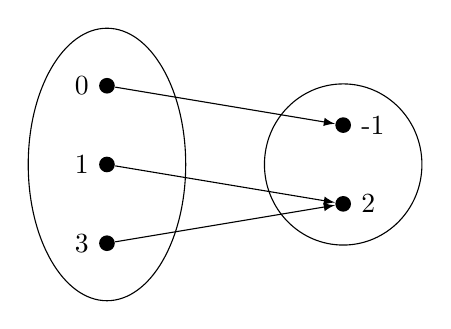
\begin{tikzpicture}
%put some nodes on the left
% \foreach \x in {1,2,3}{
% \node[fill,circle,inner sep=2pt] (d\x) at (0,\x) {};
% }

\node[fill,circle,inner sep=2pt, label={left:3}] (d1) at (0,1) {};
\node[fill,circle,inner sep=2pt, label={left:1}] (d2) at (0,2) {};
\node[fill,circle,inner sep=2pt, label={left:0}] (d3) at (0,3) {};

\node[fit=(d1) (d2) (d3),ellipse,draw,minimum width=2cm] {}; 
%put some nodes on the center
% \foreach \x[count=\xi] in {1.5,2.5}{
% \node[fill,circle,inner sep=2pt, label={}] (r1) at (2,1.5) {};
% }
\node[fill,circle,inner sep=2pt, label={right:2}] (r1) at (3,1.5) {};
\node[fill,circle,inner sep=2pt, label={right:-1}] (r2) at (3,2.5) {};

\node[fit=(r1) (r2),ellipse,draw,minimum width=2cm] {}; 

\draw[-latex] (d1) -- (r1);
\draw[-latex] (d2) -- (r1);
\draw[-latex] (d3) -- (r2);

\end{tikzpicture}
\end{center}

When defining a function $f$, we write $f:A\lthen B$, where $A$ is domain and $B$ is range

\begin{example*}
    Define the function $r:\left[-17,-\frac{\pi}{3}\right] \lthen \RR$ by the explicit formula $$r(x)=x^3,r:\left[-17,-\frac{\pi}{3}\right] \lthen \left[-17^3,-\left(\frac{\pi}{3}\right)^3\right] \subseteq \RR$$
\end{example*}

\section{Operation between functions}
Suppose $f_1, f_2$ have the same domain $A$, then we can define a new function, say $g$, to take the values of the sum of $f_1$ and $f_2$
i.e., for $f_1: A \lthen B$ and $f_2: A \lthen B$ we define $g: A \lthen B'$ bo be
$$g(x) = f_1(x) + f_2(x)\ \forall x \in A$$
Note that $B'$ might not be equal to $B$

\begin{example*}
    $f_1, f_2 : \left[0,1\right] \lthen \left[0,1\right],\ f_1(x) = x,\ f_2(x) = \frac{1}{2}x,\ g(x) = \frac{3}{2}x$ and $g: \left[0,1\right] \lthen \left[0,\frac{3}{2}\right]$
\end{example*}
For ease of notation, we write $g$ as $(f_1 + f_2)$

Similarly, we define the product function $(f_1 \cdot f_2)(x) = f_1(x)\cdot f_2(x) \ \forall x \in A$
\begin{example*}
    $f(x) = \log x$ for $x \geq 1$, $g(x) = 10x^2\ \forall x \in \RR$ 
    To define $f+g$ and $f\cdot g$, we must to the smaller domain $\{x\in\RR : x \geq 1\}$
\end{example*}

\section{Some examples of functions}

\subsection{Polynomials}
\begin{definition}
    $f: \RR \lthen \RR$ is a polynomial function, if $\exists N \in \NN$ and $\exists\{a_0, \dotsc, a_N\} \in \RR^{N+1}$ 
    $$f(x) = a_0 + a_1x+ \dotsc a_Nx^N\ \forall x \in \RR$$
\end{definition}
\subsection{Rational function}
\begin{definition}
    We say that $f$ is a rational function if for some polynomial functions $p: \RR \lthen \RR$ and $q: \RR \lthen \RR$ such that
    $$f(x) = \frac{p(x)}{q(x)}\ \forall x \in \RR\setminus R_q$$
    where $R_q = \{x\in\RR:q(x) = 0\}$ is the set of roots of $q$
\end{definition}

\subsection{Construct functions}
\begin{definition}
    $f: \RR\lthen\RR$ is a constant function if $\exists c \in \RR$ such that $f(x) = c\ \forall x \in \RR$
\end{definition}

\subsection{The identity}
\begin{definition}
    If $f(x) = x\ \forall x \in \RR$ then we say that $f$ is the identity map.
\end{definition}

\section{Composition}
\begin{definition}
    Let $f:A \lthen B$ and $g:B\lthen C$ be functions.
    We define the composition $g \circ f : A \lthen C$ by $g \circ f(x) = g(f(x))\ \forall x \in A$
\end{definition}

\section{Formal definition}
\begin{definition}\label{def:fndefine}
    A function is a collection of pairs of points with the property if $(a, b)$ and $(a, c)$ belong to the collection, the $b = c$. 
    The pairs of points are of the form $(a, f(a)$. 
    The property in \textbf{Definition~\ref{def:fndefine}} ensure that we stay clear of a confusion of the sort $f(2) = 2$ and $f(2) = 3$, which would using the diagram representation.
\begin{center}
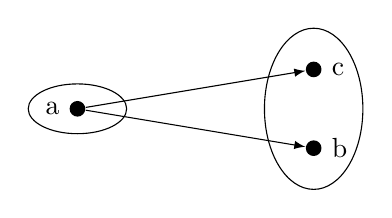
\begin{tikzpicture}
\node[fill,circle,inner sep=2pt, label={left:a}] (d2) at (0,2) {};

\node[fit=(d2),ellipse,draw,minimum width=1.25cm] {}; 

\node[fill,circle,inner sep=2pt, label={right:b}] (r1) at (3,1.5) {};
\node[fill,circle,inner sep=2pt, label={right:c}] (r2) at (3,2.5) {};
\node[fit=(r1) (r2),ellipse,draw,minimum width=1.25cm] {}; 

\draw[-latex] (d2) -- (r1);
\draw[-latex] (d2) -- (r2);

\end{tikzpicture}

\textbf{NOT} a function
\end{center}
\end{definition}

\begin{definition}
    Let $f$ be a function and denote by $\mathcal{F}$ its collection of points. The domain of $f$, written $\dom(f)$, is the set of all points $a$ such that there exists some $b$ for which $(a, b) \in \mathcal{F}$.
\end{definition}
i.e., $\dom(f) = \{a: \exists b$ for which $(a, b) \in \mathcal{F}\}$

Moreover, by \textbf{Definition~\ref{def:fndefine}} for each $a\in\dom(f)$ there exists $a$ unique $b$ such that $(a, b) \in \mathbf{F}$

\section{Graphs of functions}
An intimidate way to represent a function is by writing its coordinate pair on curves, i.e., drawing its graph

\begin{center}
    \begin{tikzpicture}
  \draw[->] (-1, 0) -- (4.2, 0) node[right] {$x$};
  \draw[->] (0, -1) -- (0, 4.2) node[above] {$f(x)$};
  \draw[scale=0.5, domain=-2:8, smooth, variable=\x] plot ({\x}, {\x*\x*0.1});
\end{tikzpicture}

This diagram is representation of $\{(x, f(x)\}, x\in A$
\end{center}

\begin{definition}
    Let $f: \RR \lthen \RR$ be a function.
    We say $f$ is \textbf{linear} if $\exists a \in \RR$ such that $$f(x) = ax,\ \forall x \in \RR$$
\end{definition}
\begin{definition}
    Let $f: \RR \lthen \RR$ be a function.
    We say $f$ is \textbf{affine} if $\exists a \in \RR$ such that $$f(x) = ax + b,\ \forall x \in \RR$$
\end{definition}\begin{definition}
    Let $f: \RR \lthen \RR$ be a function.
    We say $f$ is \textbf{even} if $\exists a \in \RR$ such that $$f(x) = f(-x),\ \forall x \in \RR$$
\end{definition}\begin{definition}
    Let $f: \RR \lthen \RR$ be a function.
    We say $f$ is \textbf{odd} if $\exists a \in \RR$ such that $$f(x) = -f(-x),\ \forall x \in \RR$$
\end{definition}

\section{What is limit}

What is a limit? Intutively, a function has a limit at a point $x_*$ if the function values $f(x)$ ``approach" this limit number as $x$ gets closer to $x_*$

\begin{center}
\begin{tikzpicture}
  \draw[->] (-1, 0) -- (4.2, 0) node[right] {$x$};
  \draw[->] (0, -1) -- (0, 4.2) node[above] {$f(x)$};
  \draw[dotted] (2, 0) -- (2, 2);
  \draw[dotted] (0, 2) -- (2, 2);
  \draw[->] (1.5, 1.35) -- (1.95, 1.8);
  \draw[->] (2.5, 2.35) -- (2.05, 1.9);
  \draw[scale=0.5, domain=-0.8:8, smooth, variable=\x] plot ({\x}, {\x});
  \node[] at (2,-0.3) {1};
  \node[] at (-0.2, 2) {1};
\end{tikzpicture}

if $f(x) = x\ \forall x \in \RR$ that as $x$ increases to $1$
\end{center}

\begin{center}
    \begin{tikzpicture}
  \draw[->] (-1, 0) -- (4.2, 0) node[right] {$x$};
  \draw[->] (0, -1) -- (0, 4.2) node[above] {$f(x)$};

  \draw[scale=0.5, domain=0.13:8, smooth, variable=\x] plot ({\x}, {1/\x});
\end{tikzpicture}

as $x \lthen \infty, f(x)$ goes arbitrary close to $0$, as $x \lthen 0, f(x)$ ``explodes" and has not limit
\end{center}

This idea of a function having a limit is also preserve for more basic objects, e.g., sequence

e.g., the sequence of points $\{0, \frac{1}{2}, \frac{2}{3}, \frac{3}{4}, \dotsc\}$ where the $n^{th}$ element of the sequnec may be written as $a_n=1-\frac{1}{n}$, converge to $1$ as $n \lthen \infty$

\subsection{definition of limit}

\begin{definition}\label{def:limit}
    Let $f: \RR \lthen \RR$ be a function and let $a, l \in \RR$.
    We say that $f$ approach the limit $l$ near $a$ if for all $\eps > 0$ there exists $\delta > 0$ such that
    $$0 < |x-a| < \delta \implies |f(x)-l| < \eps$$
    We write $\lim\limits_{x \to a} f(x) = l$
\end{definition}

Some comments on \textbf{Definition}~\ref{def:limit}
\begin{enumerate}[(i)]
    \item $\delta$ is allowed to depend on $\eps, a, l$ 
    \item ``for all $\eps > 0$" can be read as ``given any $\eps > 0$"
\end{enumerate}

\begin{example*}
    Let $f(x) = cx$ for some $c \in \RR$ we show that $\lim\limits_{x \to 1} f(x) = c$
\end{example*}
\begin{proof}
    let $\eps > 0$ be given. Then 
    \begin{align*}
        |f(x)-c|&=|cx-c|\\
        &=|c|\cdot|1-x|
    \end{align*}
    So, letting $\delta=\delta(\eps)=|c|^{-1}\cdot\eps$, we get that
    $$0 < |1-x| < \delta \implies |f(x)-c| < \eps$$
    Since this hold for all $\eps > 0$, we define $\lim\limits_{x \to 1} f(x) = c$
\end{proof}

\begin{example*}
    Let $g(x) = x\sin(\frac{1}{x})$ for some $x \in (0, \infty)$. Then $\lim\limits_{x \to 0} g(x) = 0$
\end{example*}
\begin{proof}
    Indeed, let $\eps > 0$ be given.
    Notice that $|g(x)| = |x|\cdot|\sin(\frac{1}{x})| \leq |x|$
    
    , thus, letting $\delta=\delta(\eps)=\eps$, we see that
    $$0 < |x| < \delta \implies |g(x)| < \eps$$
\end{proof}

\begin{definition}
    Let $f: \RR \lthen \RR$ and let $l \in \RR$. We say that $f$ apporaches the limit $l$ as $x$ tends to infinity if:
    for all $\eps > 0$, there exists $R > 0$ such that 
    $$x > R \implies |f(x)-l| < \eps$$
    We write $\lim\limits_{x \to \infty} f(x) = l$
    ($R$ is allowed to depend on $\eps, l$)
\end{definition}

\begin{example*}
    let $f(x) = \frac{1}{x}$ for $x > 0$. We show that $\lim\limits_{x \to \infty} f(x) = 0$

    letting $R(\eps)=\eps^{-1}$, wee see that $x > R \implies |f(x) - 0| < \eps$
\end{example*}
\begin{definition}
    Let $l \in \RR$ and $\{a_n\}_{n\in\NN}$ be a sequence of real numbers.
    We say that $a_n$ approaches the limit $l$ as $n$ tends to infinty if
    for all $\eps > 0$, there exists $N\in \NN$ such that 
    $$n > N \implies |a_n - l| < \eps$$
    Write $\lim\limits_{x \to \infty a_n }= l$
\end{definition}

\begin{example*}
    For the sequence $\{0, \frac{1}{2}, \frac{2}{3}, \frac{3}{4}, \dotsc\}$ where $a_n = 1-\frac{1}{n}\ \forall n\in\NN$
    we see that $\lim\limits_{x \to \infty a_n }= 1$
\end{example*}
\begin{proof}
    Indeed, let $\eps > 0$ be given. Observe that $|a_n - 1| < \frac{1}{n}$
    ,letting $N(\eps) = \lceil \eps^{-1}\rceil$, we see that,
    whenever $n > N$, $n > \eps^{-1} \implies \frac{1}{n} < \eps$ and $|a_n - 1| < \eps$ for such $n$
\end{proof}

What does it mean to not have a limit?

\subsection{what is no limit}
\begin{corollary}\label{def:nolimit}
   $f: \RR \lthen \RR$ does not approach the limit $l \in \RR$ at the point $a \in \RR$ if
   there exists some $\eps_0 > 0$ such that for all $\delta > 0$
   there exists $x_\delta \in \RR$ for which there holds
   \begin{center}
       $|x_\delta - a| < \delta$ and $|f(x_\delta) - l| \geq \eps_0$
   \end{center}
\end{corollary}

\begin{example*}
    We show that $\substack{f:(0, 1)\lthen (0, \infty)\\
    x\mapsto \frac{1}{x}}$ has no limit at $x=0$
\end{example*}
\begin{proof}
    We show that $\forall p \geq 0$, $f$ does not approach the limit $p$ at $x=0$
    Let $p \geq 0$ be given. We'll show that Corollary~\ref{def:nolimit} holds with $\eps_0 = 1$
    Note that $|f(x)-p| = |\frac{1}{x}-p|=\frac{1}{x} - p$ provided $0 < x \leq \frac{1}{p}$.
    Also observe that $0 < x \leq \frac{1}{p+1} \implies \frac{1}{x} - p \geq p+1-p=1$
    This given any $\delta > 0$, choosing $x_\delta=\min\{\frac{\delta}{2},\frac{1}{p+1}\}$
    we get $0 < x_\delta < \delta$ and by $|f(x_\delta - p) \geq 1$
\end{proof}

\begin{example*}
    Let $\substack{f:(0, \infty)\lthen \RR \\
    x\mapsto \sin(\frac{1}{x})}$.
    We show $f$ does not approach the value $0$ as $x \lthen 0$.
\end{example*}
\begin{proof}
    Indeed, for this case set $\eps_0 = \frac{1}{2}$ 
    and for every $\delta > 0$, set $x_\delta=\frac{1}{\frac{\pi}{2} + 2\pi n_\delta}$
    where $n_\delta \in \NN$ chosen sufficiently large such that $0 < x_\delta < \delta$.
    For instance, $n_\delta = \lceil\frac{\delta^{-1}}{2\pi}\rceil$
    clearify that $x_\delta=\frac{1}{\frac{\pi}{2} + 2\pi n_\delta} < \frac{1}{2\pi n_\delta}$ and 
    \begin{align*}
        n_\delta &\geq \frac{\delta^{-1}}{2\pi} \\
        2\pi n_\delta &\geq \delta^{-1} \\
        \frac{1}{2\pi n_\delta} &\leq \delta
    \end{align*}
    Then, $0 < x_\delta < \delta$, and 
    \begin{align*}
        f(x) &= \sin\left(\frac{1}{x_\delta}\right) \\
        &= \sin\left(\frac{\pi}{2} + \frac{1}{x_\delta}\right)\\
        &= \sin\left(\frac{\pi}{2}\right) = 1
    \end{align*}
    So, $|x_\delta - 0| < \delta$ and $f(x_\delta) - 0| = 1 > \frac{1}{2} = \eps_0$ $\left(\text{So, }\lim\limits_{x \to 0} f(x) \neq 0\right)$
\end{proof}

\begin{example}
    Let $f: \RR \lthen \RR$ be defined by
    \[ f(x) =
  \begin{cases}
    x       & \quad \text{if } x\in\QQ\\
    0  & \quad \text{if } x\notin\QQ
  \end{cases}
\]
$\lim\limits_{x \to 0} f(x) = 0$ but $f$ has no limit at any other point $a \neq 0$
\end{example}

\textbf{Fact} Given $s < t$ real numbers:
\begin{enumerate}[(i)]
    \item $\exists q \in \QQ$ such that $s < q < t$
    \item $\exists r \in \RR\setminus\QQ$ such that $s < r < t$
\end{enumerate}

\begin{proof}
    Fix $a > 0$ and let $l \in \RR$ be arbitrary. There are 2 cases
    \begin{enumerate}
        \item Suppose $l = 0$ set $\eps_0 = a$
        Then, given $\delta > 0$ by Fact(i), $\exists x_\delta \in \QQ$ such that $a < x_\delta < a + \delta$ and thus
        $|x_\delta - a| < \delta$ and $|f(x_\delta)-l| = x_\delta > a = \eps_0$
        so $f(x)\nrightarrow 0$ as $x \lthen a$
        \item Suppose $l \neq 0$ set $\eps_0=\frac{|l|}{2}$
        then given any $\delta > 0$ by Fact(ii), $\exists x_\delta\in \RR\setminus \QQ$ such that $a < x_\delta < a + \delta$, $|x_\delta - a| < \delta$ and $|f(x_\delta)-l| = |l| > \frac{|l|}{2} = \eps_0$
        repeating the same strategy for $a < 0$ concludes the proof.
    \end{enumerate}
\end{proof}

\section{Identity of Limit}
\begin{theorem}
    Let $f:\RR \lthen \RR$ and $a \in \RR$.
    Suppose that for $\mu, \nu \in \RR$ we have $\lim\limits_{x \to a} f(x) = \mu$ and $\lim\limits_{x \to a} f(x) = \nu$ then $\mu = \nu$
    (i.e., the limit is unique)
\end{theorem}
\begin{proof}
    Let $\eps > 0$ be given. 
    By the definition of the limit $\exists \delta_1 = \delta_1(\eps, a, \mu) > 0$ such that 
    $0 < |x - a| < \delta_1 \implies |f(x) - \mu| < \frac{\eps}{2}$
    also $\exists \delta_2 = \delta_2(\eps, a, \nu) > 0$ such that 
    $0 < |x - a| < \delta_2 \implies |f(x) - \nu| < \frac{\eps}{2}$
    Letting $\delta = \min\{\delta_1, \delta_2\} > 0$,
    we see that $|\mu - \nu| \leq |\mu - f(x)| + |f(x) - \nu|$, which provided $|x-a|<\delta$.
    Hence, $|\mu-\nu| < \eps$ whenever $|x-a|<\delta$

    We will show that $\mu-\nu = 0$. Suppose $\mu-\nu \neq 0$ then $|\mu-\nu| \geq 0$ but then, choosing $\eps=\frac{1}{2}|\mu-\nu|$ we get $|\mu-\nu| < \frac{1}{2}|\mu-\nu|$
    
\end{proof}


\begin{theorem}
    Let $f, g:\RR \lthen \RR$ and $a \in \RR$.
    Suppose that for $\mu, \nu \in \RR$, $\lim\limits_{x \to a} f(x) = \mu$ and $\lim\limits_{x \to a} g(x) = \nu$ then \begin{enumerate}[(a)]
        \item $\lim\limits_{x \to a} (f+g)(x) = \mu + \nu$
        \item$\lim\limits_{x \to a} (f\cdot g)(x) = \mu \cdot \nu$
    \end{enumerate}
\end{theorem}
\begin{proof}
We will prove each separately
\begin{enumerate}[(a)]
    \item Let $\eps > 0$ be given. by the definition of limit,  
    $\exists \delta_1 = \delta_1(\eps, a, \mu) > 0$ such that 
    $0 < |x - a| < \delta_1 \implies |f(x) - \mu| < \frac{\eps}{2}$ and 
    $\exists \delta_2 = \delta_2(\eps, a, \nu) > 0$ such that 
    $0 < |x - a| < \delta_2 \implies |g(x) - \nu| < \frac{\eps}{2}$.
    Let $\delta=\min\{\delta_1, \delta_2\}$, provided $0 < |x-a| < \delta$, and observe that
    \begin{align*}
        |(f+g)(x)-(\mu+\nu)| &= |(f(x)-\mu)+(g(x)-\nu)| \\
        &\leq |f(x)-\mu|+|g(x)-\nu| \\
        &< \frac{\eps}{2} + \frac{\eps}{2} = \eps
    \end{align*}
    and $0 < |x-a| < \delta \implies |(f+g)(x)-(\mu+\nu)| < \eps$
    \item Let $\eps > 0$ be given, and observe that 
    \begin{align*}
        |(f\cdot g)(x)-(\mu\nu)| &= |(f(x)g(x)-\mu g(x))+(\mu g(x)-\mu\nu)| \\
        &\leq |g(x)|\cdot|f(x)-\mu|+|\mu|\cdot|g(x)-\nu| 
    \end{align*}
    By the definition of limit $\exists \delta_g=\delta_g(\eps, a, \nu) > 0$ such that $|g(x) - \nu| < \min\{\frac{\eps}{2(1+|\mu|)}, 1\}$, whenever $0 < |x-a| < \delta_g$.
    
    Note: whenever $0 < |x-a| < \delta_g$, we have
    \begin{enumerate}[(i)]
        \item $|g(x) - \nu| < \frac{\eps}{2(1+|\mu|)}$ and $|\mu|\cdot|g(x)-\nu| < \frac{\eps}{2}$
        \item $|g(x)-\nu| < 1$ and $g(x) \leq |g(x) - \nu| + |\nu| < 1 + |\nu|$
    \end{enumerate}
    Again, by the definition of limit, $\exists\delta_f=\delta_f(\eps, a, \mu, \nu) > 0$ such that $$|x-a| < \delta_f \implies |f(x) - \mu| < \frac{\eps}{2(1+|\nu|)}$$
    then, we see that, for $\delta = \min\{\delta_f, \delta_g\}$ we have $$|(f\cdot g)(x)-(\mu\nu)| < (1 + |\nu|)\frac{\eps}{2(1 + |\nu|)} + \frac{\eps}{2} = \eps$$
\end{enumerate}
\end{proof}

\section{Infremum / Supremum}
Our objective is to give a sense of infremum/supremum as limits.
For example, consider $\left[1, 2\right]$. 
This set has the property that for every $x \in \left[1, 2\right]$, there exists a sequence of points $(x_n)_{n\in\NN}$ belonging to $\left[1, 2\right]$ such that $x_n \lthen x$ as $n \lthen \infty$.
Indeed, $x\in(1, 2)$, then for $M_x > 0$ sufficiently large. $x_n = x + \frac{1}{n\cdot M_x}$ is such that $x_n \in (1, 2)$ and $x_n \lthen x$.
And for when $x \in \{1, 2\}$, we can build the sequences $x_n = \frac{1}{100n}$ or $x_n = 2- \frac{1}{100n}$
This property also holds for $(1, 2)$, but also even though $1, 2 \notin (1, 2)$, 
there exists sequences $(y_n)_{n\in\NN}$ and $(z_n)_{n\in\NN}$ such that $y_n, z_n \notin (1, 2)\ \forall n \in \NN$ and $y_n \lthen 1$ as $n \lthen \infty$, $z_n \lthen 2$ as $n \lthen \infty$

It turns out that the property of ``having a sequence inside the set converging to this point" is a property that holds true for the $\inf$ and $\sup$ of any bounded set.

To this end, we prove the following lemma

\begin{lemma}\label{lem:bab}
    Let $B \subseteq \RR$ be a nonempty set bounded above.
    Then, given any $\eps > 0$, there exists some $b_\eps \in B$ such that $$\sup B - \eps < b_\eps\ (\leq \sup B)$$
\end{lemma}
\begin{proof}
    Let $\eps > 0$ be given. 
    Denote $\sup B$ by $\beta$.
    Suppose for contradiction that no such $b_\eps$ exists, Then for all $b \in B$, 
    we must have $b \leq \beta - \eps$ but then $\beta - \eps$ is the least upper bound for $B$
\end{proof}

An analogous argument prove
\begin{lemma}\label{lem:bbl}
    Let $A \subseteq \RR$ be a nonempty set bounded below.
    Then, given any $\eps > 0$, there exists some $a_\eps \in B$ such that $$(\inf A \leq)\ a_\eps < \inf A + \eps$$
\end{lemma}

\begin{corollary}
    Let $A\subseteq \RR$ be nonempty and bounded, then, $\exists(x_n)_{n\in\NN}$ and $\exists(y_n)_{n\in\NN}$ 
    for which $x_n, y_n \in A$ for all $n \in \NN$ and
    $\lim\limits_{x \to \infty}x_n = \inf A$, $\lim\limits_{x \to \infty}y_n = \sup A$
\end{corollary}
\begin{proof}
    By Lemma~\ref{lem:bab} for each $n \in \NN$, $\exists y_n \in A$ such that $\sup A - \frac{1}{n} < y_n \leq \sup A$ and 
    $|y_n - \sup A| < \frac{1}{n} \lthen 0$ as $n \lthen \infty$
    So, $\lim\limits_{x \to \infty}y_n = \sup A$.
    Also, for each $n \in \NN$, by Lemma~\ref{lem:bbl}, $\exists x_n \in A$ such that $\inf A \leq x_n < \inf A + \frac{1}{n}$.
    i.e., $|x_n - \inf A| < \frac{1}{n} \lthen 0$ as $n \lthen \infty$. 
    So, $\lim\limits_{x \to \infty}x_n = \inf A$.
\end{proof}

\begin{lemma}
    Suppose $A$ is non-empty and bounded below.
    Let $B$ be the set of all lower bounds of $A$.
    Then $\inf A = \sup B$
\end{lemma}
\begin{proof}
There are 3 steps

\par\textbf{Step 1} $\left[B\text{ is nonempty}\right]$ 
Since $A$ is bounded below, there exists at least one lower bound, which belongs to $B$, so $B \neq \emptyset$

\par\textbf{Step 2} $\left[B\text{ is bounded above}\right]$ 
Suppose for contradiction that $B$ is not bounded above. 
Then given any $n \in \NN, \exists x_n \in B$ such that $x_n \geq n$.
Then by the definition of $B$, $x_n$ is a lower bound for $A$ for each $n \in \NN$.
Thus given any $a \in A$, we have $a \geq x_n \geq n\ \forall n \in \NN$.
Here $B$ is bounded above.

\par\textbf{Step 3} $\left[\text{showing the equality}\right]$ 
\begin{itemize}
    \item[$(\leq)$] Let $\nu = \inf A$ nad $\mu = \sup B$.
    Since $\nu$ is the infimum of $A$, $\nu$ is a lower bound for $A$.
    So $\nu \in B \implies \nu \leq \sup B = \mu$ 
    \item[$(\geq)$] Let $\eps > 0$ be arbitrary. Then by \textbf{Lemma}~\ref{lem:bab} $\exists b_\eps \in B$ such that $\mu - \eps < b_\eps \leq \mu$.
    Hence, $\mu < \eps + b_\eps$. Now, let $a \in A$ be any point of $A$ and observe that since $b_\eps \in B$, $b_\eps \leq a \implies \mu < \eps + b_\eps \leq \eps + a$.
    i.e., $\mu < \eps + a$ for all $a \in A$.
    i.e., $\mu - \eps < a\ \forall a \in A$.
    So, $\mu - \eps$ is a lower bound for $A \implies \mu - \eps < \inf A = \nu$
    i.e., $\mu < \nu + \eps$, but $\eps > 0$ was arbitrary $\implies \mu \leq \nu$
\end{itemize}

\end{proof}

\chapter{Continuous Function}

What does it mean for a function to be continuous?

Infinitely, this is some smoothness to the function i.g.,

\begin{center}
\begin{tikzpicture}
  \draw[->] (-1, 0) -- (4.2, 0) node[right] {$x$};
  \draw[->] (0, -1) -- (0, 4.2) node[above] {$f_1(x)$};
  \draw[scale=0.5, domain=-0.8:8, smooth, variable=\x] plot ({\x}, {\x});
\end{tikzpicture}

\begin{tikzpicture}
  \draw[->] (-1, 0) -- (4.2, 0) node[right] {$x$};
  \draw[->] (0, -1) -- (0, 4.2) node[above] {$f_2(x)$};
  \draw[-] (-0.5, 2) -- (0.5, 2);
  \draw[-] (0.5, 2) -- (1.5, 3);
  \draw[-] (1.5, 3) -- (2.5, 3);
  \draw[-] (2.5, 3) -- (3.5, 1.2);
  \draw[-] (3.5, 1.2) -- (4, 1);
\end{tikzpicture}
\end{center}

But, on the other hand 

\begin{center}
\begin{tikzpicture}
  \draw[->] (-1, 1) -- (4.2, 1) node[right] {$x$};
  \draw[->] (0, -1) -- (0, 4.2) node[above] {$f_3(x)$};
  \draw[-] (-0.5, 0) -- (1, 0);
  \draw[-] (1, 2) -- (4, 2);
  % \node[circle, draw] at (1, 0){};
  \node at (1, 0)[circle,fill,inner sep=1.5pt]{};
  \node at (1, 2)[draw,circle,fill=white,minimum size=4pt,inner sep=1.5pt]{};
\end{tikzpicture}
\end{center}

is not continuous

\section{Definition of Continuous Function}
\begin{definition}\label{def:contin}
    Let $f: \RR \lthen \RR$. We say $f$ is continuous at the point $x_0 \in \RR$ if there holds $\lim\limits_{x \to x_0}f(x) = f(x_0)$
\end{definition}

\begin{remark*}
    For $f$ to be continuous at $x_0 \in \RR$, we require
    \begin{enumerate}[(i)]
        \item $\lim\limits_{x \to 0} f(x)$ exists
        \item $\lim\limits_{x \to 0} f(x) = f(x_0)$
    \end{enumerate}
\end{remark*}

Another way of writing Definition~\ref{def:contin} is
\begin{definition*}[32]
    $f$ is continuous at $x_0$ if for all $\eps > 0$, $\exists\delta=\delta(\eps, x_0, f(x_0)) > 0$ such that
    $$|x-x_0| < \delta \implies |f(x) - f(x_0)| < \eps$$
\end{definition*}

\begin{example*}
    $f_3$ is not continuous at the point $x = 1$. 
\end{example*}
\begin{proof}
    Indeed, setting $\eps_0 = 1$, 
    we see that, given any $\delta > 0$, the point $x_\delta = 1 + \frac{\delta}{2}$ is such that $|x_\delta - 1| < \delta$ and $|f(x_\delta) - f(1)| = |1-(-1)|=2 > \eps_0$
\end{proof}

\begin{example*}
    $f(x) = x^2$ is continuous.
\end{example*}
\begin{proof}
    Indeed, let $x_0 \in \RR$ be any point and observe that
    \begin{align*}
        |f(x) - f(x_0)| &= |x^2-x_0^2| \\
        &= |(x+x_0)(x-x_0)| \\
        &= |x+x_0|\cdot|x-x_0|
    \end{align*}
    Let $\eps > 0$ be given. Now let $\delta = \min\left\{1, \frac{\eps}{2(1+|x_0|)}\right\}$, then
     \begin{align*}
        |x+x_0| &= |x-x_0+2x_0| \\
        &\leq |x-x_0| + 2|x_0| \\
        &\leq 1 + 2|x_0|
    \end{align*}
    Then provided $|x - x_0| < \delta$ we get
    $$|f(x) - f(x_0)| \leq (1 + 2|x_0|)\cdot\frac{\eps}{2(1 + |x_0|)} < \eps$$
\end{proof}
\begin{example*}
\[ f(x) =
  \begin{cases}
    0       & \quad  x = 0\\
    x \sin\left(\frac{1}{x}\right)  & \quad x \neq 0
  \end{cases}
\]
$f$ is continuous at $x = 0$
\end{example*}
\begin{proof}
    Indeed, let $\eps > 0$ be given and observe that 
    \begin{align*}
        |f(x) - f(0)| &= |x|\cdot\left|\sin\left(\frac{1}{x}\right)\right| \text{ for } x \neq 0 \\
        & \leq |x|
    \end{align*}
    So, letting $\delta(\eps) = \frac{\eps}{2}$, we see that
    $$|x-0| < \delta \implies |f(x)-f(0)| \leq \frac{\eps}{2} < \eps$$
\end{proof}

\section{Identity of Continuous Function}

\begin{lemma}
    Let $f, g: \RR \lthen \RR$ be continuous at $a \in \RR$. Then
    \begin{enumerate}[(i)]
        \item $f+g$ is continuous at $a$
        \item $f\cdot g$ is continuous at $a$
    \end{enumerate}
\end{lemma}
\begin{proof}
    We will prove each separately
    \begin{enumerate}[(i)]
        \item let $\eps > 0$ be given. By the definition of continuous, $\exists \delta_f = \delta_f(\eps, a) > 0$ such that 
        $$|x-a| < \delta_f \implies |f(x) - f(a)| < \frac{\eps}{2}$$
        and, $\exists \delta_g = \delta_g(\eps, a) > 0$ such that 
        $$|x-a| < \delta_g \implies |g(x) - g(a)| < \frac{\eps}{2}$$
        So, letting $\delta = \min\{\delta_f, \delta_g\}$, suppose $|x-a| < \delta$, we see that 
        \begin{align*}
            |f(x) + g(x) - (f(a) + g(a))| &\leq |f(x) - f(a)| + |g(x) - g(a)| \\
            &= \frac{\eps}{2} + \frac{\eps}{2} \\
            &= \eps
        \end{align*}
        \item let $\eps$ be given. Note that
        $$|f(x)g(x)-f(a)g(a)| \leq |g(x)|\cdot|f(x)-f(a)| + |f(a)|\cdot|g(x)-g(a)|$$
        Since $g$ is continuous at $a$, $\exists \delta_g = \delta_g(\eps, a) > 0$ such that
        $$|x-a| < \delta_g \implies |g(x)-g(a)| < \min\left\{1, \frac{\eps}{2(1 + |f(a)|)}\right\}$$
        Then, provided $|x-a| < \delta_g$, we get 
        $$|g(x)| \leq \overbrace{|g(x)-g(a)|}^{<1} + |g(a)| < 1 + |g(a)|$$
        Also, since $f$ is continuous at $a$, $\exists \delta_f = \delta_f(\eps, a) > 0$ such that
        $$|x-a| < \delta_f \implies |f(x) - f(a)| < \frac{\eps}{2(1 + |g(a)|)}$$
        Then, letting $\delta = \min\{\delta_f, \delta_g\}$, we see that whenever $|x-a| < \delta$, we have form
        $$|f(x)g(x) - f(a)g(a)| < (1 + |g(a)|)\left(\frac{\eps}{2(1 + |g(a)|)}\right) + |f(a)|\cdot\frac{\eps}{2(1 + |f(a)|)} < \eps$$
    \end{enumerate}
\end{proof}

\begin{lemma}
    Let $g: \RR \lthen \RR$ be continuous at $a \in \RR$ and $f: \RR \lthen \RR$ be continuous at $g(a)$. 
    Then $f \circ g$ is continuous at $a$
\end{lemma}

\begin{proof}
    Let $\eps > 0$ be given. Since $f$ is continuous at $g(a)$, $\exists \delta_f = \delta_f(\eps, a) > 0$ such that 
    $$|y - g(a)| < \delta_f \implies |f(y) - f(g(a))| < \eps$$
    Meanwhile, $g$ is continuous at $a$, so $\exists \delta_g = \delta_g(\delta_f(\eps, a), a) > 0$ such that
    $$|x - a| < \delta_g \implies |g(x) - g(a)| < \delta_f$$
    So, letting $\delta = \delta_g$, we see that
    \begin{align*}
        |x-a| < \delta &\implies |g(x) - g(a)| < \delta_f \\
        &\implies |f(g(x)) - f(g(a))| < \eps
    \end{align*} 
\end{proof}

\begin{lemma}
    Let $f: \RR \lthen \RR$ be continuous at $a$, and suppose $f(a) > 0$. 
    Then $\exists \delta > 0$ such that $f(x) > 0\ \forall x \in \left[a - \delta, a + \delta\right]$
\end{lemma}

\begin{proof}
    Since $f$ is continuous at $a$, $\exists \delta_f = \delta_f(a, \overbrace{f(a)}^\eps) > 0$ such that
    $$|x-a| < \delta_f \implies |f(x) - f(a)| < \overbrace{\frac{1}{2}f(a)}^\eps$$
    It follows that, for $x \in (a - \delta_f, a + \delta_f)$, we have
    \begin{align*}
        f(x) &= (f(x) - f(a)) + f(a) \\
        &\geq f(a) - |f(x) - f(a)| \\
        &> f(a) - \frac{1}{2}f(a) \\
        &= \frac{1}{2}f(a) > 0
    \end{align*}
    In turn, letting $\delta = \frac{1}{2}\delta_f$, we see that $f(x) > 0\ \forall x \in \left[a - \delta, a + \delta\right]$
\end{proof}


\section{Definition of Left/Right Continuity}

$f$ continuous on $(a, b)$ if $f$ is continuous at $x$, for all $x \in (a, b)$.
What does it mean for $f$ to be continuous at on $\left[a, b\right]$?
Should there be a difference between ``continuous on $(a, b)$" and ``continuous on $\left[a, b\right]$".

To gather intution, let's look at $f(x) = \frac{1}{x}$ on $(0, 1)$ and $\left[0, 1\right]$.

\begin{center}
    \begin{tikzpicture}
      \draw[->] (-1, 0) -- (4.2, 0) node[right] {$x$};
      \draw[->] (0, -1) -- (0, 4.2) node[above] {$f(x)$};
      \draw[scale=1, domain=0.3:3.5, smooth, variable=\x] plot ({\x}, {1/\x});
    \end{tikzpicture}
\end{center}

It's clar that $f$ is continuous at every point $a \in (0, 1)$ but $\lim\limits_{x \to 0}f(x)$ is not defined.
So, it ought to not be continuous on $\left[0, 1\right]$
We make the following define

\begin{definition*}[32]
    Let $f: \RR \lthen \RR$ and $a < b$ be real numbers.
    \begin{enumerate}[(i)]
        \item We say f is continuous on $(a, b)$ if $f$ is continuous at $x$ for every $x \in (a, b)$
        \item We say $f$ is continuous on $\left[a, b\right]$ if $f$ is continuous on $(a, b)$ and 
        $\lim\limits_{x \to a^+}f(x) = f(a)$ and $\lim\limits_{x \to b^-}f(x) = f(b)$
    \end{enumerate}
    We write $\lim\limits_{x \to a^+} f(x)$ to mean ``The limit $f$ as $x$ tends to $a$ from above''
    also written $\lim\limits_{x \searrow a} f(x)$
    and $\lim\limits_{x \to b^-} f(x)$ to mean ``The limit $f$ as $x$ tends to $b$ from below''
    also written $\lim\limits_{x \nearrow a} f(x)$
\end{definition*}

\begin{definition*}[32]\label{def:lfcts}
    Let $f: \RR \lthen \RR$ and $a \in \RR$
    \begin{enumerate}[(i)]
        \item We write $\mu = \lim\limits_{x \searrow a} f(x)$ if for all $\eps > 0$, $\exists\delta > 0$ such that
        whenever $a < x < a + \delta$ we have $|\mu - f(x)| < \eps$
        \item We write $\nu = \lim\limits_{x \nearrow a} f(x)$ if for all $\eps > 0$, $\exists\delta > 0$ such that
        whenever $a  - \delta< x < a$ we have $|\nu - f(x)| < \eps$
    \end{enumerate}
\end{definition*}
\begin{example*}
    Considered this graph 
    \begin{center}
        \begin{tikzpicture}
            \draw[-] (-1, 0) -- (1, 0) node[right] {};
            \draw[-] (4, 0) -- (6, 0) node[left] {};
            \node at (1, 1)[circle,fill,inner sep=1.5pt]{};
            \node at (4, 2)[circle,fill,inner sep=1.5pt]{};
            \node at (1, 0)[draw,circle,fill=white,minimum size=4pt,inner sep=1.5pt]{};
            \node at (4, 0)[draw,circle,fill=white,minimum size=4pt,inner sep=1.5pt]{};
            \draw (1, 1) sin (2, 2) cos (2.5, 1.5) sin (3, 1) cos (4, 2);
            \node[] at (1,-0.3) {$a$};
            \node[] at (4,-0.3) {$b$};
            \node[] at (0,1) {$f(a) = 1$};
            \node[] at (5,2) {$f(b) = 2$};
        \end{tikzpicture}
    \end{center}
    then, $\lim\limits_{x \searrow a} f(x) = 1$ and $\lim\limits_{x \nearrow b} f(x) = 2$
    on the other hand $\lim\limits_{x \nearrow a} f(x) = 0$ and $\lim\limits_{x \searrow b} f(x) = 0$
\end{example*}
\begin{example*}
    $\lim\limits_{x \to x_0} f(x)$ exists $\iff$ $\lim\limits_{x \nearrow x_0} f(x)$ and $\lim\limits_{x \searrow x_0} f(x)$ exists and are equal.
\end{example*}
    

\section{3 Hard Theorems}

\begin{theorem}[Intermediate Value Theorem]\label{thm:ivalt}
    Let $f: \RR \lthen \RR$ be continuous on $\left[a, b\right]$ for $a < b$.
    Suppose $f(a) < 0 < f(b)$
    Then $\exists \xi \in (a, b)$ such that $f(\xi)=0$
\end{theorem}

\begin{theorem}\label{thm:upbndcts}
    Let $f: \RR \lthen \RR$ be continuous on $\left[a, b\right]$ for $a < b$.
    Then $f$ is bounded above on $\left[a, b\right]$, i.e., $\exists M \in \RR$ such that $f(x) \leq M\ x \in \left[a, b\right]$
\end{theorem}

\begin{theorem}\label{thm:supbndcts}
    Let $f: \RR \lthen \RR$ be continuous on $\left[a, b\right]$.
    Then $\exists \xi \in \left[a, b\right]$ such that $f(x) \leq f(\xi)\ \forall x \in \left[a, b\right]$
    i.e., $f(\xi)=\sup\{f(x): x\in\left[a, b\right]\}$
    (we say that $f$ achieves its supremum on $\left[a, b\right]$)
\end{theorem}

\begin{lemma*}[$35'$]
    Let $f: \RR \lthen \RR$ and $b \in \RR$.
    Suppose $\lim\limits_{x \nearrow b} f(x) = f(b) > 0$
    Then $\exists \delta > 0$ such that $f(x) > 0$ for all $x \in (b - \delta, b)$
\end{lemma*}

\begin{proof}
    Directly from Definition 32(ii) (definition of $\lim\limits_{x \nearrow b} f(x)$) such that
    $$x \in (b - \delta, b) \implies |f(x) - f(b)| < \frac{1}{2} f(b)$$
    Then for such $x \in (b - \delta, b)$ we have 
    \begin{align*}
        f(x) &= (f(x) - f(b)) + f(b) \\
        & \geq f(b) - \overbrace{|f(x) - f(b)|}^{<\frac{1}{2}f(b)} \\
        &> \frac{1}{2} f(b) > 0
    \end{align*}
    Hence, for $x \in \left(b - \frac{\delta}{2}, b\right)$ we have $f(x) > 0$
\end{proof}

\begin{lemma*}[$35''$]
    Let $f: \RR \lthen \RR$ and $b \in \RR$.
    Suppose $\lim\limits_{x \searrow a} f(x) = f(a) > 0$
    Then $\exists \delta > 0$ such that $f(x) > 0$ for all $x \in (a, a + \delta)$
\end{lemma*}

\begin{proof}[Proof Theorem \ref{thm:ivalt}]
    Define the set $A=\{x \in \left[a, b\right]:f(y) < 0\ \forall y \in \left[a, x\right]\}$
    Since $f(a) < 0$, so $a \in A$, so $A \neq \emptyset$
    Also, using Lemma $35''$ $\exists \delta_1 > 0$ such that $f(y) < 0\ \forall y \in \left[a, a + \delta_1\right]$
    so $a + \delta_1 \in A$, and by Lemma $35'$ 
    $\exists \delta_2 > 0$ such that $f(y) > 0\ \forall y \in \left[b-\delta_2, b\right]$ where $b-\delta_2$ is an upper bound for $A$.
    So $A$ is bounded above and $\sup A$ is well-defined.
    Let $\alpha=\sup A$. We already know that $\alpha\in (a, b)$
    our aim is to show that $f(\alpha) \neq 0$
    We proceed by contradiction: 
    
    Suppose for contradiction that $f(\alpha) \neq 0$
    There are 2 possibilities
    \begin{enumerate}[(i)]
        \item $f(\alpha) < 0$
        \item $f(\alpha) > 0$
    \end{enumerate}
    Suppose (i) holds, Since $\alpha \in (a, b)$ and $f(\alpha) < 0$
    by \textbf{Lemma 35}, $\exists \delta_3 > 0$ such that $f(y) < 0\ \forall y \in \left[\alpha - \delta_3, \alpha + \delta_3\right]$
    But then $\alpha + \delta_3 \in A$ and $\alpha + \delta_3 > \alpha$

    Suppose (ii) holds. Then since $\alpha \in (a, b)$, $f(\alpha) > 0$ and $f$ is continuous. By \textbf{Lemma 35}, $\exists \delta_4 > 0$ such that $f(x) > 0\ \forall x \in \left[\alpha - \delta_4, \alpha+\delta_4\right]$
    But then $\alpha = \sup A$ by \textbf{Lemma 28} $\exists x_0 \in A$ such that $\alpha - \frac{\delta_4}{2} < x_0$
    Thus $x_0 \in (\alpha-\frac{\delta_4}{2}, \alpha) \subseteq \left[\alpha - \delta_4, \alpha+\delta_4\right] \implies f(x_0) > 0$
    But $x_0 \in A$ so $(f_x) < 0$
\end{proof}

\begin{corollary}
    Let $f: \RR \lthen \RR$ be continuous on $\left[a, b\right]$ and let $c\in\RR$.
    Suppose $f(a) < c < f(b)$. Then $\exists\xi \in (a, b)$ such that $f(\xi)=c$
\end{corollary}
\begin{proof}
    Define $g(x) = f(x) - c$ and apply \textbf{Theorem}~\ref{thm:ivalt} to $g$
\end{proof}

\begin{example}
    Let $f(x) = x^4 + x - 3\ \forall x \in \RR$
    \textbf{Fact}: all polynomials are continuous $\forall x \in \RR$
    A nice application of the Intermidiate Value Theorem is to find roots of continuous functions
    We can see by plugging in that 
    $$ f(1) = 1 + (-1) - 3 = -3$$
    $$ f(2) = 16 + 2 - 3 = 15$$
    IVT $\implies \exists x_0 \in (1, 2)$ such that $f(x_0) = 0$
    This  at least lets us estimate where roots are
\end{example}

\begin{example}
    Let $f(x) = x^4 + x - 3 + \tan\left(\frac{x}{2}\right)$ (continuous on $(-\pi, \pi)$)
    $$f(-1) = -3 - \tan\left(\frac{1}{2}\right) < 0$$
    $$f(2) = 15 - \tan\left(\frac{1}{2}\right) > 0$$
    IVT $\implies \exists x_0 \in (-1, 2)$ such that $f(x_0) = 0$
\end{example}


What is it useful for?
If we look at the set $f(\left[a, b\right]) = \{f(x) : x \in \left[a, b\right]\}$
and Theorem~\ref{thm:upbndcts} tell us that set is bounded.
Since the set is bounded, it has a supremum.
You can think of this as ``local max'' of $f$ on the interval $\left[a, b\right]$

Before proving Theorem~\ref{thm:upbndcts}, let's look at one of its consequences.

\begin{corollary}
    Let $f: \RR \to \RR$ be continuous on $\left[a, b\right]$.
    Then $f$ is bounded below on $\left[a, b\right]$, i.e.,
    $\exists m \in \RR$ such that $m \leq f(x)\ \forall x \in \left[a, b\right]$
\end{corollary}
\begin{proof}
    Since $f$ is continuous, so is $(-f)$. Now apply Theorem~\ref{thm:upbndcts} to $-f$.
    $\exists M \in \RR$ such that $-f(x) \leq M\ \forall x \in \left[a, b\right]$
    the, $f(x) \leq -M\ \forall x \in \left[a, b\right]$
\end{proof}

\textbf{Takeaway}: If $f$ is continuous on $\left[a, b\right]$, then $f$ is bounded above + below on $\left[a, b\right]$

To prove Theorem~\ref{thm:upbndcts}, we'll need a few Lemmas.
\begin{lemma}
    Let $f: \RR \to \RR$ is continuous at $a \in \RR$, then $\exists \delta > 0$ such that
    $f$ is bounded above on the interval $\left[a-\delta, a + \delta\right]$
\end{lemma}
\begin{proof}
    Since $f$ is continuous at $a$, $\exists \delta = \delta(a, \overbrace{1}^\eps)$ such that 
    $|x-a| < \delta \implies |f(x) - f(a)| < 1$
    This for such $x$ we have 
    \begin{align*}
        f(x) &= f(x) - f(a) + f(a) \\
        &\leq |f(x) - f(a)| + |f(a)| \\
        &< 1 + |f(a)|
    \end{align*}
    For $x$ satisfying $|x-a| < \delta$, we have $f(x) < 1 + f(a)$.

    In particular, $f(x) < 1 + f(a)\ \forall x \in \left[a-\frac{\delta}{2}, a + \frac{\delta}{2}\right]$ 
\end{proof}

\begin{lemma*}($43'$)
    Let $f: \RR \to \RR$ be a function and $b \in \RR$.
    Suppose $\lim\limits_{x \nearrow b} f(x) = f(b)$. 
    Then $\exists \delta > 0$ such that $f$ is bounded above on $\left[b-\delta, b\right]$
\end{lemma*}

\begin{proof}
    By Definition $32''$, $\exists \delta = \delta(b, 1)$ such that
    $$0 < |x-b| < \delta \implies |f(x) - f(b)| < 1$$
    Therefore, for such $x$, 
    \begin{align*}
        f(x) &= f(x) - f(b) + f(b) \\
        &\leq |f(x) - f(b)| + |f(b)| \\
        &< 1 + |f(b)|
    \end{align*}
    $f(x) < f(b) + 1\ \forall x \in \left[b-\frac{\delta}{2}, b\right]$
\end{proof}

\begin{lemma*}($43''$)
    Let $f: \RR \to \RR$ be a function and $a \in \RR$.
    Suppose $\lim\limits_{x \searrow a} f(x) = f(a)$. 
    Then $\exists \delta > 0$ such that $f$ is bounded above on $\left[a, a+\delta\right]$
\end{lemma*}

\begin{proof}[Proof Theorem~\ref{thm:upbndcts}]
    As in the proof of Theorem~\ref{thm:ivalt}, consider the set
    $$A = \{ x \in \left[a, b\right] : f \text{ is bounded above on }\left[a, x\right]\}$$
    Since $a \in A$, we know $a \neq \emptyset$.
    Moreover, the point $b$ is an upper bound for $A$, so $\sup A = \alpha$ exists.

    Our objective is to show that $\alpha = b$.

    Suppose for contradiction that $\alpha < b$.
    (Note that we must have $a < \alpha$.
    We can't have $a > \alpha$ since $a \in A$. and $\sup A \geq a$.
    If $\alpha = a$, then $A = \{a\}$, but we know from Lemma $43''$ that
    $\exists \delta > 0$ such that $\left[a, a+\delta\right] \subseteq A$)

    By assumption $a < \alpha < b$ and so Lemma $43$ $\implies \exists\delta > 0$ such that
    $f$ isbounded on $\left[\alpha - \delta, \alpha + \delta\right]$.
    Let's say $f(x) \leq m_2$ on this interval $\left[\alpha - \delta, \alpha + \delta\right]$.

    By Lemma 28 (Alternate definition of supremum)
    $\exists x_0 \in A$ such that $\alpha - \delta < x_0 \leq \alpha$.
    $f$ is bounded above on $\left[a, x_0\right]$ (by the definition of $A$).
    say $f(x) \leq m_1$ on $\left[a, x_0\right]$
    \begin{center}
    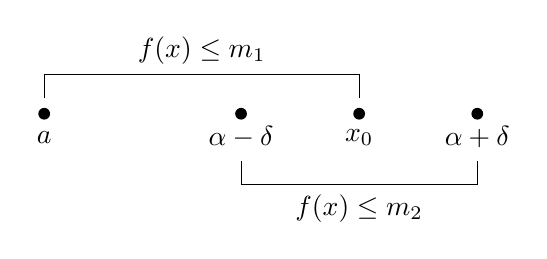
\begin{tikzpicture}
        \draw[-] (0, 0.5) -- (4, 0.5);
        \draw[-] (0, 0.5) -- (0, 0.2);
        \draw[-] (4, 0.5) -- (4, 0.2);
        \node at (2, 0.8) {$f(x) \leq m_1$};
        \node at (0, 0)[circle,fill,inner sep=1.5pt]{};
        \node at (0, -0.3){$a$};
        \node at (2.5, 0)[circle,fill,inner sep=1.5pt]{};
        \node at (2.5, -0.3){$\alpha - \delta$};
        \node at (4, 0)[circle,fill,inner sep=1.5pt]{};
        \node at (4, -0.3){$x_0$};
        \node at (5.5, 0)[circle,fill,inner sep=1.5pt]{};
        \node at (5.5, -0.3){$\alpha + \delta$};
        \draw[-] (2.5, -0.9) -- (5.5, -0.9);
        \draw[-] (2.5, -0.9) -- (2.5, -0.6);
        \draw[-] (5.5, -0.9) -- (5.5, -0.6);
        \node at (4, -1.2) {$f(x) \leq m_2$};
    \end{tikzpicture}
    \end{center}
    Thus, $f(x) \leq \max\{m_1, m_2\}\ \forall x \in \left[a, \alpha+\delta\right]$
    We deduce that $\alpha + \delta \in A$ and $\alpha + \delta > \alpha = \sup A$.
    Hence, 
    \begin{align*}
        \alpha = b &\iff \sup A = b \\
        &\implies f \text{ is bounded above on }\left[a, b\right] \text{ for every } x < b \text{ \circled{1}}
    \end{align*}
    Finally, using continuity at the point $b$ by Lemma $43'$ $\exists \delta'$ such that
    $f$ is bounded on $\left[b-\delta', b\right]$ \circled{2}.

    Hence, choosing $x = b - \delta'$ in \circled{1}, $\exists M$ such that $f(x) \leq M,\ \forall x \in \left[a, b - \delta'\right]$.
    and by \circled{2}, $\exists M_2$ such that $f(x) \leq M_2,\ \forall x \in \left[b-\delta', b\right]$.
    So, $f(x) \leq \max\{M, M_2\}\ \forall x \in \left[a, b\right]$.
\end{proof}

Summarize steps:
\begin{enumerate}[(i)]
    \item define a good set $A$
    \item show $b = \sup A$
    \item show $b \in A$
\end{enumerate}

The picture is 
\begin{center}
    \begin{tikzpicture}
        \draw[->] (-1, 0) -- (4.2, 0) node[right] {$x$};
        \draw[->] (0, -1) -- (0, 4.2) node[above] {$f(x)$};
        \draw[dotted] (-0.5, 3.2) -- (3.5, 3.2);
        \draw[-] (0.5, -0.1) -- (0.5, 0.1);
        \draw[-] (3.5, -0.1) -- (3.5, 0.1);
        \node at (0.5, -0.3){$a$};
        \node at (3.5, -0.3){$b$};
        \node at (-0.8, 3.2){$M$};
        \draw[dotted] (-0.5, -0.6) -- (3.5, -0.6);
        \node at (-0.8, -0.6){$m$};
        \draw (0.5, 1) sin (1.5, 3) cos (2, 1.25) sin (2.5, -0.5) cos (3.5, 2);
    \end{tikzpicture}
\end{center}

Whenever $f$ is continuous on $\left[a, b\right], \exists M > m$ such that 
$m \leq f(x) \leq M\ \forall x \in \left[a, b\right]$

\textbf{Note:} We must be careful aboue being continuous on $\left[a, b\right]$,
and mot just $(a, b)$. Indeed, $\substack{f:(0, 1)\lthen (0, \infty)\\
x\mapsto \frac{1}{x}}$, $f$ is continuous on $\left[\tilde{x}, \infty\right)$ for every $\tilde{x} > 0$,
but it is \underline{not} continuous on $\left[0, \infty\right)$.
    
\textbf{Question:} does these exists $\xi_1,\xi_2 \in \left[a, b\right]$ such that

$$f(\xi_1) = \inf_{\left[a, b\right]} f \text{ and } f(\xi_2) = \sup_{\left[a, b\right]} f$$

\textbf{Anwer:} Yes

Later on, when we discuss differentiability, if $\sup$/$\inf$ is achieved in $(a, b)$,
then $f' = 0$ at such points. This we will prove later. 

\begin{proof}[Proof of Theorm~\ref{thm:supbndcts}]
    We already know from Theorem~\ref{thm:upbndcts} that $f$ is bounded on $\left[a, b\right]$,
    i.e., the set $B = f(\left[a, b\right]) = \{f(x): x \in \left[a, b\right]\}$ is bounded.
    This set is nonempty and so $\beta = \sup B$ is well-defined;
    Since $\beta \geq f(x)\ \forall x \in \left[a, b\right]$ it suffies to show that
    $\exists \xi \in \left[a, b\right]$ such that $f(\xi) = \beta$.
    
    Suppose for contradiction that this is not the case, i.e., 
    $\beta \neq f(y)\ \forall y \in \left[a, b\right]$ Then the function $g: \left[a, b\right] \to \RR$,
    defined by $g(x) = \frac{1}{\beta - f(x)} \forall x \in \left[a, b\right]$,
    is well-defined and $g$ is continuous on $\left[a, b\right]$ by virtue of Lemma 33

    Since $g$ is continuous, by Theorem~\ref{thm:upbndcts}$\implies\ g$ is bounded above on $\left[a, b\right]$
    However, by Lemma 28, given any $n \in \NN, \exists x_n \in \left[a, b\right]$ such that 
    $$\beta - \frac{1}{n} < f(x_n)\leq \beta \implies g(x_n) \geq \frac{1}{\beta - \left(\beta-\frac{1}{n}\right)} = n$$ 

    Hence given any $n \in \NN, \exists x_n \in \left[a, b\right]$ such that $g(x_n) \geq n$ and
    therefore $g$ is unbounded on $\left[a, b\right]$.
\end{proof}

We've actually proved
\begin{corollary}\label{col:44}
    Let $f: \RR \to \RR$ be continuous on $\left[a, b\right]$. Then $\exists\xi \in \left[a, b\right]$ such that
    $f(\xi) = \sup\{f(x) : x \in \left[a, b\right]\}$ (we often write with the shorthand $\sup_{\left[a, b\right]} f$)
\end{corollary}

\begin{corollary}
    Let $f: \RR \to \RR$ be continuous on $\left[a, b\right]$. Then $\exists \xi \in \left[a, b\right]$ such that
    $f(\xi) = \inf\{f(x) : x \in \left[a, b\right]\}$ 
\end{corollary}

\begin{proof}
    Apploy Corollary~\ref{col:44} to the function $-f$ and use the result $\inf B = -\sup(-B)$.
\end{proof}

\section{Usage of 3 Hard Theorem}

\begin{example}
    Suppose $f, g$ are continuous on $\left[a, b\right]$ and $f(a) < g(a)$ and $f(b) > g(b)$.
    Then $\exists x \in \left[a, b\right]$ such that $f(x) = g(x)$ (in actual fact, $x \in (a, b)$)
\end{example}

\begin{proof}
    define $h(x) = f(x) - g(x)$. Then $h$ is continuous on $\left[a, b\right]$,
    $h(a) < 0 < h(b)$ so from Theorem~\ref{thm:ivalt}, $\exists \xi \in (a, b)$ such that
    $h(\xi) = 0 \implies f(\xi)=g(\xi)$
\end{proof}

\begin{example}
    Suppose $f: \RR \to \RR$ is continuous on $\left[0, 1\right]$ and suppose 
    $0 \leq f(x) \leq 1\ \forall x \in \left[0, 1\right]$. Then $\exists x_0 \in \left[0, 1\right]$ 
    such that $f(x_0) = x_0$ (we can imagine that $f$ cross $y = x$)
\end{example}

\begin{proof}
    Note that if $f(0) = 0$ on if $f(1) = 1$, then we are done.
    Suppose that $f(0) \neq 0$ and $f(1) \neq 1$ then $0 < f(0)$ and $f(1) < 1$
    Let $g(x) = x - f(x)$. Then, $g(0) = 0 - f(0) < 0$ and $g(1) = 1 - f(1) > 0$.
    So, $g$ is continuous and $g(0) < 0 < g(1)$, where Theorem~\ref{thm:ivalt} 
    $\exists x_0 \in \left[0, 1\right]$ such that $g(x_0) = 0$ and hence $x_0 =f(x_0)$
\end{proof}

\begin{example}
    There are 3 sub-examples here:
    \begin{enumerate}[(a)]
        \item Suppose $f: \RR \to \RR$ satsfies $|f(x)| \leq |x|$ for all $x \in \RR$. Then $f$ is continuous at $0$
        \item There exists a function which satisfies the assumption of a.) but is not continuous at any other points
        other than $x = 0$
        \item Suppose $g$ is continuous at $0$ and $g(0) = 0$ and suppose $|f(x)| \leq |g(x)|\ \forall x \in \RR$.
        Then $f$ is continuous at $0$.
    \end{enumerate}
\end{example}

\begin{proof}
    We will prove each separately:
    \begin{enumerate}[(a)]
        \item The inequallity implies $f(0) = 0$. Let $\eps > 0$ be given, then the inequallity show that
        $$|f(x) - f(0)| = |f(x)| \leq |x - 0|$$
        so letting $\delta = \eps$, we see that
        $$|x-0| < \delta \implies |f(x) - f(0)| < \eps$$
        so $f$ is continuous at $0$
        \item \[ f(x) =
            \begin{cases}
            x       & \quad \text{if } x \in \QQ \\
            0       & \quad \text{if } x \notin \QQ
            \end{cases}
        \]
        Then $|f(x)| \leq |x|\ \forall x$ but $f$ is not continuous at any points other than $0$
        \item Since $g(0) = 0$, we immediately get $f(0) = 0$. Let $\eps > 0$ be given.
        Since $g$ is continuous at $0$, $\exists \delta = \delta(\eps, 0) > 0$ such that
        $$|x - 0| < \delta \implies |g(x) - g(0)| \leq \eps$$
        but then, in view of the bound $|f(x)| \leq |g(x)|\ \forall x$, we see that
        $$|x - 0| < \delta \implies |f(x) - f(0)| = |f(x)| \leq |g(x)| = |g(x)-g(0)| < \eps$$
    \end{enumerate} 
\end{proof}

\begin{example}
    This exercis is here to help us gain more familiarity with limits-- it's not concern with 
    continuous functions per se.
    \begin{enumerate}[(i)]
        \item Let $f, g: \RR \to \RR$ and suppose $f(x) \leq g(x)\ \forall x \in \RR$ and suppose 
        $\mu := \lim\limits_{x\to a} f(x), \nu := \lim\limits_{x\to a}g(x)$
        Show that $\mu \leq \nu$
        \item Now suppose $f(x) < g(x)\ \forall x \in \RR$. Does this guarantee $\mu < \nu$?
    \end{enumerate}
\end{example}

\begin{proof}
    We will prove each separately:
    \begin{enumerate}[(i)]
    \item Let $\eps > 0$ be given. Then $\exists \delta_1 = \delta_1(\eps, a, \mu) > 0$ and 
        $\exists \delta_2 = \delta_2(\eps, a, \nu) > 0$ such that 
        $$ |x-a| < \delta_1 \implies |f(x) - \mu| < \frac{\eps}{2},$$ 
        $$ |x-a| < \delta_2 \implies |g(x) - \nu| < \frac{\eps}{2}$$
        Set $\delta := \min(\delta_1, \delta 2)$
        Then, provided $|x-a| < \delta$, we have 
        \begin{align*}
            \nu - \mu &= (\nu - g(x)) + (g(x) - f(x)) + (f(x) - \mu) \\
            &\geq \underbrace{g(x) - f(x)}_{\geq 0} - \underbrace{|\nu - g(x)|}_{<\frac{\eps}{2}} - \underbrace{|\mu - f(x)|}_{<\frac{\eps}{2}} \\
            &> -\eps
        \end{align*}
        So, $\nu - \mu > -\eps$ for all $\eps > 0 \implies \nu - \mu \geq 0$
    \item \underline{NO}: Suppose $f(x) = 0$ and $g(x) = \begin{cases}
        1       & \quad \text{if } |x| < 1\\
        \frac{1}{x}& \quad \text{if } |x| \geq 1
        \end{cases}$

        Then $\lim\limits_{x\to \infty} f(x) = 0$ and $\lim\limits_{x\to \infty} g(x) = 0$
    \end{enumerate}
\end{proof}

\begin{example}
    Let $f(x) = \begin{cases}
        \sin\left(\frac{1}{x}\right)       & \quad \text{for } x \neq 0\\
        0 & \quad x = 0
        \end{cases}$
    \begin{enumerate}[(a)]
        \item Show that $f$ is not continuous on $\left[-1, 1\right]$
        \item Show that $f$ satisfies the conclusion of Theorem~\ref{thm:ivalt} (IVT)
    \end{enumerate}
\end{example}

\begin{proof}\text{ }
    \begin{enumerate}[(a)]
        \item for every $\delta > 0$, $n_\delta := \max\left(\left\lceil\frac{1}{2\pi}\delta^{-1}\right\rceil, 1\right)\in \NN$ such that 
        $$\frac{1}{\frac{\pi}{2} + 2\pi n_\delta} < \delta\text{ and }x_\delta := \frac{1}{\frac{\pi}{2} + 2\pi n_\delta}$$
        we get $0 < x_\delta < \delta$ and 
        $$|f(x_\delta) - f(0)| = \left|\sin\left(\frac{\pi}{2} + 2\pi n_\delta\right)\right| = 1$$
        so, for all $\delta > 0, \exists x_\delta$ such that $0 < x_\delta < \delta$ and
        $|f(x_\delta) - f(0)| = 1$, so $f$ is not continuous at $0$.
        \item $f$ is not continuous at $0$, however $f$ is continuous on $(-1, 0)$ and on $\left(0, 1\right]$ and 
        so Theorem~\ref{thm:ivalt} holds on any interval of the form $\left[-1, y\right]$ and $\left[ x, 1\right]$ for 
        $y < 0$ and $x > 0$

        It remains to check that 

        *Suppose $a > 0$ and $f(a) > 0$. Then, for every $c \in \left[0, f(a)\right], \exists \xi_c\in\left[0, a\right]$ such that 
        $f(\xi_c) = c$

        Note that $f(a) \leq 1$, Indeed $\xi = \frac{1}{\arcsin(c)}$ is such that 
        \begin{align*}
            f(\xi) &= c \\
            \sin\left(\frac{1}{\xi}\right) &= \sin(\arcsin(c))
        \end{align*}
        So the only remaining issue is that we do not necessarily have $\xi \in \left[0, a\right]$.

        To this end, notice that, for every $N \in \NN$, $\xi = \frac{1}{2\pi N + \arcsin(c)}$ 
        also satisfies $f(\xi) = c$ and hence, choosing $N$ sufficiently large such that $\frac{1}{2\pi N + \arcsin(c)} \leq a$, 
        we have that $\xi = \frac{1}{2\pi N + \arcsin(c)}$ is a point that verifies *
    \end{enumerate}
\end{proof}

\begin{example}
    Suppose $f, g: \RR \to \RR$ are continuous, and $f(x)^2 = g(x)^2\ \forall x \in \RR$ and $f(x) \neq 0$. 
    Then either
    \begin{enumerate}[(i)]
        \item $f(x) = g(x)\ \forall x \in \RR$
        \item $f(x) = -g(x)\ \forall x \in \RR$
    \end{enumerate}
    i.e., $f$ cannot `jump' between $\pm g$.
\end{example}

\begin{proof}
    Suppose for contradiction that $\exists a, b \in \RR$ such that $f(a) = g(a)$ and $f(b) = -g(b) \circledast$
    and wlog(without loss of generality), assume $a < b$.
    Since $f(x) \neq 0\ \forall x$, we also assume wlog $f(a) < 0$
    Then it can't be the case that $f(b) > 0$. 
    Indeed, if this were the case, then by Theorem~\ref{thm:ivalt},
    $\exists \xi \in (a, b)$ such that $f(\xi) = 0$, which contradicts $f(x) \neq 0\ \forall x$.

    Hence $f(a) < 0$ and $f(b) < 0$. 
    
    Then, $\circledast \implies g(a) < 0$ and $g(b) > 0$, 
    so Theorem~\ref{thm:ivalt}$\implies \exists \zeta \in (a, b)$ such that $g(\zeta) = 0$.
    But then $f(\zeta) = 0$, which is again a contradiction.
\end{proof}

\begin{example}
    Suppose $f: \RR \to \RR$ is continuous and such that $f(x)^2 = x^2\ \forall x \in \RR$.
    Then, either $f(x) = x\ \forall x \in \RR$, or $f(x) = -x\ \forall x \in \RR$, or $f(x) = |x|\ \forall x \in \RR$.
\end{example}

\begin{proof}
    It sufficies to show that 
    \begin{enumerate}[(A)]
        \item for $x < 0$, either: $f(x) = x\ \forall x < 0$, or $f(x) = -x\ \forall x < 0$
        \item for $x > 0$, either: $f(x) = x\ \forall x > 0$, or $f(x) = -x\ \forall x > 0$
    \end{enumerate}
    We only prove (B), as the proof for (A) is identical.

    Suppose for contradiction $\exists 0 < a < b$ such that (wlog) $f(a) = -a$ and $f(b) = b$.
    Then, observe that $f(a) < 0$, while $f(b) > 0$.

    Thus, Theorem~\ref{thm:ivalt} $\implies \exists \xi \in (a, b)$ such that $f(\xi) = 0$.
    But, $(f(\xi))^2 = \xi^2 > a^2 > 0$
\end{proof}

\begin{example}
    Suppose $f$ is continuous on $\left[a, b\right]$ and $f(x) \in \QQ\ \forall x \in \left[a, b\right]$.
    Then, $f$ is a constant function, i.e., $\exists q \in \QQ$ such that $f(x) = q\ \forall x \in \left[a, b\right]$.
\end{example}

\begin{proof}
    Suppose for contradiction that $f$ is not constant, i.e., $\exists a, b \in \RR$ such that $f(a) < f(b)$ and wlog $a < b$.
    Since between any 2 real numbers, there exists an innational number, it follows that there exists $c \in \RR \setminus \QQ$ such that $f(a) < c < f(b)$.

    Then, from IVT, $\exists \xi_c \in (a, b)$ such that $f(\xi_c) = c \in \RR \setminus \QQ$.
\end{proof}

\begin{example}
    Suppose $f$ is continuous on $\left[0, 1\right]$ and $f(0) = f(1)$. Let $n \in \NN$ be arbitrary.
    Then, $\exists x_* \in \left[0, 1\right)$ such that $f(x_*) = f\left(x_* + \frac{n}{n+1}\right)$. 
\end{example}

\begin{proof}
    Define $g: \left[0, 1 - \frac{1}{n}\right] \to \RR$ by $g(x) := f(x) - f\left(x + \frac{1}{n}\right)$.

    Suppose for contradiction that $g(x) \neq 0\ \forall x \in \left[0, 1 - \frac{1}{n}\right]$.
    By cty (using Theorm~\ref{thm:ivalt}), we must have either $g(x) > 0$ or $g(x) < 0\ \forall x \in \left[0, 1 - \frac{1}{n}\right]$.

    Wlog, assume $g(x) > 0\ \forall x \in \left[0, 1 - \frac{1}{n}\right]$.
    Then, $f(x) > f\left(x + \frac{1}{n}\right)\ \forall x \in \left[0, 1 - \frac{1}{n}\right]$.
    It follows that, by setting $x=0$, $f(0) > f\left(\frac{1}{n}\right)$, but also by setting $x = \frac{1}{n}$,
    $$f\left(\frac{1}{n}\right) > f\left(\frac{2}{n}\right), \ldots, f\left(\frac{m}{n}\right) > f\left(\frac{m + 1}{n}\right)\ \forall m \in \left\{0, \ldots, \frac{n-1}{n}\right\}$$
    $$\implies f(0) > f\left(\frac{1}{n}\right) > f\left(\frac{2}{n}\right), \ldots, f\left(\frac{n-1}{n}\right) > f\left(1\right)$$
    $$\implies f(0) > f(1)$$
    but we assumed $f(0) = f(1)$, which is a contradiction.
\end{proof}

\begin{example}
    Suppose $\phi : \RR \to \RR$ is continuous and $n \in \NN$, and $\lim\limits_{x \to \infty}\frac{\phi(x)}{x^n} = 0 = \lim\limits_{x \to -\infty}\frac{\phi(x)}{x^n}$.
    Then,
    \begin{enumerate}[(a)]
        \item if $n$ is odd, $\exists x_* \in \RR$ such that $(x_*)^n + \phi(x_*) = 0$
        \item if $n$ is even, $\exists y \in \RR$ such that $(y)^n + \phi(y) \leq x^n + \phi(x)\ \forall x \in \RR$
    \end{enumerate}
\end{example}

\begin{proof}
    Define $\psi: \RR \to \RR$ by $\psi(x):= x^n + \phi(x)\ \forall x \in \RR$
    and note that $\psi$ is also continuous on $\RR$.
    % Then, $\psi(x) < -\frac{1}{2}(R_1)^n\ \forall x < -R_1$.
    \begin{enumerate}[(a)]
        \item Since $n$ is odd, $\lim\limits_{x\to -\infty}\frac{\psi(x)}{|x|^n} = -1 + \underbrace{\lim\limits_{x \to -\infty} \frac{\phi(x)}{|x|^n}}_{=0}$
        and similarly $\lim\limits_{x\to \infty}\frac{\psi(x)}{|x|^n} = 1$.

        Note that $x \mapsto \frac{\psi(x)}{|x|^n}$ is continuous on any internal excluding 0. 

        Then, since $\frac{\psi(x)}{|x|^n}$ is continuous on $(-\infty, 0)$, $\exists R_1 = R_1(\frac{1}{2}) > 0$ such that
        $$x < -R_1 \implies \left|\frac{\psi(x)}{|x|^n} - (-1)\right| < \frac{1}{2}$$
        i.e., for $x < -R_1$, we have $\frac{\psi(x)}{|x|^n} < (-1) + \frac{1}{2} = -\frac{1}{2}$.
        $$\implies \psi(x) < -\frac{1}{2}|x|^n\ \forall x \in \RR$$

        i.e., for all $x < -R_1$, we have $\psi(x) < 0\ \circledast$.

        Similarly, $\exists R_2 = R_2(\frac{1}{2}) > 0$ such that 
        \begin{align*}
            x > R_2 &\implies \left|\frac{\psi(x)}{|x|^n}  - 1\right| < \frac{1}{2} \\
            &\implies \psi(x) > |x|^n > \frac{1}{2}\ \forall x > R_2 \\
        \end{align*}
        Therefore, $\psi(x) > 0$ for all $x > R_2\ \circledast \circledast $.

        By $\circledast$ and $\circledast \circledast$,$\exists a, b \in \RR$ $(a < b)$ such that
        $$\psi(a) < 0 < \psi(b)$$ Then since $\psi$ is continuous, by Theorem~\ref{thm:ivalt}
        $\implies \exists x_* \in (a, b)$ suc htaht $\phi(x_*) = 0$, i.e., $x_*^n + \phi(x_*) = 0$.
    \end{enumerate}
\end{proof}

\begin{example}
    
\end{example}
\begin{example}
    
\end{example}
\begin{example}
    
\end{example}

\begin{example}
    Suppose $f$ is continuous and $\circledast \lim\limits_{x \to -\infty} f(x) = \lim\limits_{x \to \infty} f(x) = 0$, 
    and $f(x) > 0\ \forall x \in \RR$. Then, $\exists x_* \in \RR$ such that $f(x) \leq f(x_*)\ \forall x \in \RR$.
\end{example}

\begin{proof}
    Let $\mu := \displaystyle\max_{y \in \left[-1, 1\right]} f(y)$, by $\circledast$, $\exists R_1, R_2 > 0$ such that
    $$x < -R_1 \implies 0 < f(x) < \frac{1}{2} \mu$$ 
    $$x > R_2 \implies 0 < f(x) < \frac{1}{2} \mu$$ 

    Hence $0 < f(x) < \frac{1}{2} \mu$ for all $|x| \in \RR := \max\{R_1, R_2\}$.
    and meanwhile $\displaystyle\sup_{x \in \RR} f(x) \geq \displaystyle\sup_{x \in \left[-1, 1\right]} f(x) = \mu$.

    $\displaystyle\sup_{x \in \RR} f(x)$ is well-defined Since $\sup_{\left[-R, -R\right]} f $ is well-defined and achieved by Theorem and 
    $|f(x)| < \frac{1}{2}\mu$ for $|x| > R$.

    $$ + \infty > \sup_{x \in \RR} f(x) \geq \max_{x \in \left[-R, R\right]} f(x) \geq \mu > \sup_{|x| > R} f(x)$$

    It follows that $\sup_{x\in\RR} f(x) = \sup_{x \in \left[-R, R\right]} f(x)$
    $(\RR = \underbrace{\{x : |x| \leq R\}}_{=\left[-R, R\right]} \cup \{x : |x| > R\})$

    Since $f$ is continuous, it achieves its boundes by Theorem 38
    $\implies \exists x_* \in \left[-R, R\right]$ such that $f(x_*) = \sup_{\left[-R, R\right]} f = \sup_{\RR} f$.
\end{proof}

\begin{example}
    Let $f: \RR \to \RR$ be defined by 
    $$f(x) = (\sin x)^2 + (\sin (x + (\cos x)^7))^2$$
    Then, $\exists c > 0$ such that $f(x) \geq c\ \forall x \in \RR$.
\end{example}

\begin{proof}
    Observe that $f(x) \geq 0\ forall x$ and $A := \{ f(x) : x\in \RR\}$ is bounded below by 0.

    Define $c := \inf A$ is well-defined. 
    \begin{align*}
        f(x + 2\pi) &= (\sin (x + 2\pi))^2 + \sin (\overbrace{(x + 2\pi) + (\underbrace{\cos (x + 2\pi)}_{=\cos x})^7}^{=x + 2\pi + (\cos x)^7})^2 \\
        &= (\sin x)^2 + \sin (x + (\cos x)^7)^2 \\
        &= f(x)
    \end{align*}

    $f$ is $2\pi$-periodic, 
    $\implies c = \inf A = \inf\{f(x): x \in \left[0, 2\pi\right]\}$

    Since $f$ is continuous, Theorem 38 $\implies \exists x_* \in \left[0, 2\pi\right]$ such that $f(x_*) = c$.
    
    Suppose for contradiction that $c = 0$
    \begin{align*}
        &\implies f(x_*) = 0 \\
        &\implies (\underbrace{\sin x_*}_{=0})^2 + (\underbrace{\sin (x_* + (\cos x_*)^7)}_{=0})^2 = 0 \\
        &\implies x_* \in \{0, \pi, 2\pi\}\text{ but then }\cos x_* \in \{1, -1\} \\
        &\implies x_* + (\cos x_*)^7 \in \{1, \pi-1, 2\pi + 1\} \\
        &\implies \sin(x_* + (\cos x_*)^7) \in \{\sin(1), \sin(\pi - 1)\} \text{ neither of which are } 0\\
    \end{align*} 
\end{proof}

\section{Uniform Continuity}

Finally, we look at uniform continuity

\begin{definition} \label{def:uniform}
    Let $f: \RR \to \RR$. We say $f$ is \underline{uniformly continuous} on an interval $A$ if
    for all $\eps > 0, \exists \delta = \delta(\eps) > 0$ such that 
    $$|x - y| < \delta\text{ and } x, y \in A \implies |f(x) - f(y)| < \eps$$
    \underline{\textbf{KEY}}: $\delta$ is \underline{not} depend on a specific point. 
\end{definition}

\begin{example*}
    $f(x) = x$ is uniformly continuous on $\RR$. 
    Let $\eps > 0$ be given then letting $\delta = \eps$, we see that 
    $$|x-y| < \delta \implies |f(x) - f(y)| < \eps$$
\end{example*}

\begin{example*}\label{ex:xsq}
    $f(x) = x^2$ is \underline{not} uniformly continuous on $\RR$.
\end{example*}

Fix $\eps > 0$ and recall from Lecture 10 that
$$|f(x) - f(x_0)| = |x^2 - x_0^2| = |x - x_0||x + x_0|$$
and so we need $\delta = \min\left(1, \frac{\eps}{1 + 2|x_0|}\right)$
to have $|x-x_0| < \delta \implies |f(x) - f(x_0)| < \eps$.

We see that $\delta$ depends on specific point $x_0$.

This is only an indication that $f$ is not uniformly continuous -- not a proof yet.


The negation of Definition~\ref{def:uniform}

\begin{definition*}[$61'$]
    $\exists \eps_0 > 0$ such that for all $\delta > 0$ there exist corresponding $x_\delta, y\delta \in A$ such that
    $$|x_\delta - y_\delta| < \delta\text{ and } |f(x_\delta) - f(y_\delta)| \geq \eps_0$$
\end{definition*}

\begin{proof}[Proof of Example~\ref{ex:xsq}]
    Let $\eps_0 = 1$. Observe that for $x > y > 0$,
    $$|f(x) - f(y)| = x^2 - y^2 = (x+y)(x-y)$$
    For each $\delta > 0$ choose $y_\delta = \delta^{-1}$ and $x_\delta = \delta^{-1} + \frac{\delta}{2}$

    Then, $x_\delta + y_\delta = 2\delta^{-1} + \frac{\delta}{2} > 2\delta^{-1}$ and
    $|x_\delta - y_\delta| =\frac{\delta}{2} < \delta$. 

    Hence, $|x_\delta - y_\delta| < \delta$ and also 
    \begin{align*}
        |f(x_\delta) - f(y_\delta)|&= (x_\delta + y_\delta)(x_\delta - y_\delta) \\
        &= (2\delta^{-1} + \frac{\delta}{2})\cdot\frac{\delta}{2} \\
        &= 1 + \frac{\delta^2}{4} \\
        &> 1 = \eps_0
    \end{align*}
\end{proof}

\begin{remark*}
    $x \mapsto x^2$ is uniformly continuous on $\left[-1, 1\right]$, even though it is not uniformly continuous on $\RR$. 
\end{remark*}

\begin{example}
    Let $f: \left[0, \infty\right) \to \left[0, \infty\right), x \mapsto x^{\frac{1}{2}}$ 
    Then $f$ is uniform continuous on $\left[0, \infty\right)$.
\end{example}

\begin{proof}
    Let $x, y \in \left[0, \infty\right)$ and wlog assume $x > y$. Notice that 
    $$\oplus |f(x) - f(y)| = \sqrt{x} - \sqrt{y} \overbrace{\leq}^{\circledast } \sqrt{x-y}$$
    Hence, given any $\eps > 0, |x-y| < \eps^2 \underbrace{\implies}_{\oplus} |f(x) - f(y)| < \eps$.

    \underline{proof of $\circledast$}: let $a > b \geq 0$
    \begin{align*}
    (\sqrt{a} - \sqrt{b})^2 &= a + b \overbrace{- 2\sqrt{a}\sqrt{b}}^{ < -2\sqrt{b}\sqrt{b} = -2b} \\
    &\leq a - b \\
    \implies \sqrt{a} - \sqrt{b} &\leq \sqrt{a - b}
    \end{align*}
\end{proof}

\begin{theorem}
    If $f$ is continuous on $\left[a, b\right]$, then $f$ is uniformly continuous on $\left[a, b\right]$.
\end{theorem}

The choice of the interval $A$ matters on the Definition~\ref{def:uniform}.

\begin{example}
    \text{ }
    \begin{enumerate}[(i)]
        \item $f(x) = \sin\left(\frac{1}{x}\right)$ is continuous and bounded on $\left(0, 1\right]$ however it it not uniformly continuous on $\left(0, 1\right]$.
        \item $f(x) = \sin\left(e^x\right)$ is continuous and bounded on $\left[0, \infty\right)$ however it is not uniformly continuous on $\left[0, \infty\right)$. 
    \end{enumerate}
\end{example}
\chapter{Differenitiation}

Office hours on Monday

\begin{enumerate}
  \item Office hour 6.pm to 7.pm on Monday
  \item can meet before 8:50 am Monday in my office Van Vleck 613 (send an email on sunday)
\end{enumerate}

Consider a function defined on on interval $I$, with real values.
$f: I \to \RR$

\begin{definition*}
  $f$ is differentiable at the point $a \in I$ if the limit $\lim\limits_{x \to a} \frac{f(x) - f(a)}{x - a}$  exists,
  then we call this limit the deriviative $f'(a)$
\end{definition*}

\begin{center}
  \begin{tikzpicture}
    \draw[->] (-1, 0) -- (4.2, 0) node[right] {$x$};
    \draw[->] (0, -1) -- (0, 4.2) node[above] {$f(x)$};
    \draw[scale=1, domain=0.3:3.5, smooth, variable=\x] plot ({\x}, {\x^2/4});

    \draw[dotted] (2, -0.5) -- (2, 4) node[above] {$$};
    \draw[dotted] (2.5, -0.5) -- (2.5, 4) node[above] {$$};
    \draw[-] (2, 1) -- (2.5, 1) node[above] {$$};
    \draw[-] (2.5, 1) -- (2.5, 1.5625) node[above] {$$};
    \node[] at (2.25,0.8) {$x-a$};
    \node[] at (4,1.25) {$f(x) - f(a)$};
    \node[] at (2,-0.2) {$a$};
    \node[] at (2.5,-0.2) {$x$};
  \end{tikzpicture}

  $y = f(x)$, $\frac{f(x) - f(a)}{x-a} = $ slope of $f$
\end{center}

Computation of some derivatives

\begin{example*}
  \text{ }
  \begin{enumerate}[(i)]
    \item $f(x) = c$ ($c$ is some fixed point)
      we get $f'(a) = 0$ for all $a$, 

      $f(x) = f(a) = 0$ for all $x$, $\frac{f(x) - f(a)}{x-a} = 0 \implies f$ is differentiable and $f'(a) = 0$ for all $a$

      $\lim\limits_{x \to a} \frac{f(x) - f(a)}{x-a} = f'(x)$ is equivalent with saying $\lim\limits_{h \to 0} \frac{f(a+h) - f(a)}{h} = f'(a)$
    \item $f(x) = x$, then $$\frac{f(a+h) - f(a)}{h} = \frac{a + h - a}{h} = 1$$ (written $f'(x) = 1$)

    \item $f(x) = x^2$, then fix $a$, $$\frac{f(a + h) - f(a)}{h} = \frac{(a+h)^2 - a^2}{h} = \frac{a^2 + 2ah + h^2 - a^2}{h} = 2a + h$$
    $$\lim\limits_{h \to 0} \frac{f(a+h) - f(a)}{h} = \lim\limits_{h \to 0}2a + h = 2a$$
    \item $f(x) = |x|$, We should examine the differentiability of $f$ at \underline{$a = 0$}
    $$\frac{f(0 + h) - \overbrace{f(0)}^{=0}}{h} = \frac{|h|}{h} =\begin{cases}
      1       & \quad \text{if } h > 0\\
      -1  & \quad \text{if } h < 0
    \end{cases}$$
    The limit does not exist, and thus $f$ is not differentiable at $0$.
    \item $f(x) = \sqrt{|x|}$, $f$ is not differentiable at $0$ because $f(0) = 0$ and $\frac{f(0 + h) - f(0)}{h} = \frac{\sqrt{|h|}}{h}$, this limit also does not exist 

    Examine differentiability and derivative of $f(x) = \sqrt{|x|}$ at $x = a, a > 0$
    \begin{align*}
    \frac{f(a + h) - f(a)}{h} &= \frac{\sqrt{|a + h|} - \sqrt{|a|}}{h} \\
    &= \frac{\sqrt{a + h} - \sqrt{a}}{h} \\
    &= \frac{a+h - a}{\sqrt{a + h} + \sqrt{a}}\cdot \frac{1}{h} \\
    &= \frac{1}{\sqrt{a + h} + \sqrt{a}} \to \frac{1}{2\sqrt{a}}\\
    \end{align*}
    \item $f(x) = x^n$ 
    $$\frac{f(a+h) - f(a)}{h} = \frac{(a + h) ^ n - a^n}{h} = n\cdot a^{n-1}$$
  \end{enumerate}
\end{example*}

\section{Basic fact about differentiation}

Continuity is necessary (but not sufficient) for differentiation 

\begin{theorem*}
  If $f: I \to \RR$ is differentiable at $a$ the $f$ is continuous at $a$.
\end{theorem*}

\textbf{Reminder} If $\lim\limits_{x \to a} F(x) = l$ and $\lim\limits_{x \to a} G(x) = m$, then $\lim\limits_{x \to a} F(x)G(x)= lm$

If $\lim\limits_{x \to a} F(x) = l$ and $\lim\limits_{x \to a} G(x) = m$, then $\lim\limits_{x \to a} \frac{F(x)}{G(x)}= \frac{l}{m}$ or not? Yes if $m \neq 0$

\begin{proof}
  We know that $\lim\limits_{x \to 0} \frac{f(a + h) - f(a)}{h} = f'(a)$
  $$f(a + h) - f(a) = \frac{f(a + h) - f(a)}{h} \cdot h$$
  $$\implies \lim\limits_{h \to 0} f(a + h) - f(a) = f'(a) \cdot 0 = 0$$
  $$\lim\limits_{h \to 0} f(a + h) = f(a)$$ 
  this is continuity of $f$ at $a$
  
  Another argument : for sufficiently small $h$, $|f(a + h) - f(a)| \leq C|h|$
\end{proof}

\section{Sum Rule}

\begin{theorem*}
  Let $f: I \to \RR$ and $g: I \to \RR$, $a\in I$ assume that $f$ and $g$ are differentiable at $a$. 
  Then $f + g$, $(f + g)(x) = f(x) + g(x)|_{x = a}$ is differentiable and its derivative $f'(a) + g'(a)$
  (The derivative of the sum is the sum of the derivatiives)
\end{theorem*}

\begin{proof}
  \begin{align*}
    \frac{(f+g)(a + h) - (f+g)(a)}{h} &= \frac{f(a + h) + g(a + h) - (f(a) + g(a))}{h} \\
    &= \frac{f(a + h) - f(a)}{h} + \frac{g(a + h) - g(a)}{h} \\
  \end{align*}
  As $h \to 0$ this has limit $f'(a) + g'(a)$
\end{proof}

\section{Product Rule}

\begin{theorem*}
  Let $f: I \to \RR$ and $g: I \to \RR$, $a\in I$ assume that $f$ and $g$ are differentiable at $a$. 
  the $f\cdot g$ is differentiable at $a$
  $$(f\cdot g)'(a) = f'(a)g(a) + f(a)g'(a)$$
\end{theorem*}
\begin{proof}
  \begin{align*}
    \frac{f(a + h)g(a + h) - f(a)g(a)}{h} &= \frac{(f(a+h) - f(a))g(a+h) + f(a)g(a+h) - f(a)g(a)}{h} \\
    &= \underbrace{\frac{f(a+h) - f(a)}{h}}_{f'(a)}\cdot \underbrace{g(a+h)}_{\to g(a)} + \underbrace{\frac{g(a + h) - g(a)}{h}}_{\to g'(a)} \cdot \underbrace{f(a)}_{f(a)} \\
  \end{align*}
  By theorem about products and of limits, and the continuity of $g$ at $a$, we get

  $$\lim\limits_{h \to 0} \frac{f(a+h)g(a+h) - f(a)g(a)}{h} = f'(a)g(a) + g'(a)f(a)$$
\end{proof}


\begin{theorem*}
  Let $f: I \to \RR$ and $g: I \to \RR$, $a\in I$ is differentiable at $a$, and if $g(a) \neq 0$
  then $\frac{1}{g}$ is differentiable at $a$ and $$\left(\frac{1}{g}\right)'(a) = -\frac{g'(a)}{(g(a))^2}$$
  % $$\left(\frac{f}{g}\right)'(a) = \frac{f'g - fg'}{g^2} |_a$$
\end{theorem*}
\begin{proof}
  \begin{align*}
    \frac{\frac{1}{g(a+h)} - \frac{1}{g(a)}}{h} &= \frac{g(a) - g(a + h)}{g(a+h)g(a)}\cdot\frac{1}{h} \\
    &= \frac{1}{g(a+h)g(a)}\cdot (-1)\frac{g(a+h) - g(a)}{h} \\
    &\to \frac{1}{(g(a))^2}\cdot (-1) g'(a) 
  \end{align*}
\end{proof}


\section{Quotient Rule}
\begin{theorem*}
  Let $f: I \to \RR$ and $g: I \to \RR$, $a\in I$ assume $f$ and $g$ are differentiable at $a$, and if $g(a) \neq 0$
  then $\frac{f}{g}$ is differentiable at $a$ and $$\left(\frac{f}{g}\right)'(a) = \frac{f'(a)g(a) - f(a)g'(a)}{g(a)^2}$$
\end{theorem*}
\begin{proof}
  Combine the theorems about products and reciprocals of differentiable function

  \begin{align*}
  \left(\frac{f}{g}\right)'(a) &= \left(f \cdot \frac{1}{g}\right)'(a) \\
  &= f'(a) \cdot \frac{1}{g(a)} + f(a) \cdot \left(\frac{1}{g}\right)'(a) \\
  &= \frac{f'(a)}{g(a)} + f(a)\left(-\frac{g'(a)}{g(a)^2}\right) \\
  &= \frac{f'(a)g(a) - f(a)g'(a)}{g(a)^2}
  \end{align*}
\end{proof}

\begin{example*}
  \begin{align*}
    \left(\frac{\sin x}{\cos x}\right)' &= \frac{\sin'(x) \cos(x) - \cos' x \sin x}{(\cos x)^2} \\
    &= \frac{(\cos x)^2 - (-\sin ^2 x)}{(\cos x)^2} \\
    &= \frac{1}{(\cos x)^2} \\
  \end{align*}
\end{example*}

\begin{example*}
  $f(x) = x^n$ then
  $f'(x) = n x^{n-1}$
\end{example*}
\begin{proof}
  $$f_0(x) = 1, f_0'(x) = 0$$
  $$f_1(x) = x, f_1'(x) = 1$$
  $$f_1(x) = x^2, f_2'(x) = 2x$$
  We want to show this formula for a given $n$, assuming that we already know if for $n = 1$,
  In other words, the formula $f_{n-1}'(x) = (n-1)x^{n-1}, n \geq 2$,
  implies the formula for $f_n$

  Induction step: $$f_n(x) = x^n = \underbrace{x^{n-1}}_{f_{n-1}} \cdot \underbrace{x}_{f_1}$$
  By using Product Rule, we get
  \begin{align*}
  f_n'(x) &= f_{n-1}'(x)f_1(x) + f_{n-1}(x)f_1'(x) \\
  &= (n-1)x^{n-1} \cdot x + x^{n-1} \cdot 1 \\
  &= nx^{n-1} 
  \end{align*}
\end{proof}

\begin{example*}
  \begin{align*}
    (fg)'' &= (f'g + fg')' \\
    &= (f'g)' + (fg')' \\
    &= f''g + f'g' + f'g' + fg'' \\
    &= f''g + 2f'g' + fg'' \\
  \end{align*}
  $(fg)''' = f'''g + 3f''g' + 3f'g'' + fg'''$
  and can be written as $(fg)^{(3)}$
  $$(fg)^{(n)}(x) = \sum_{k=0}^n \binom{n}{k} f^{(k)}(x)g^{(n-k)}(x)$$
  As the analogy
  $$(a + b)^n = \sum_{k=0}^n \binom{n}{k} a^k b^{n-k}$$
\end{example*}

We will not talk much about higher derivative in this class

\section{Chain Rule}

Let $\zeta(x) = f(g(x))$
Assume that $g$ is defined on an interval containing $a$, and $g$ is differentiable at \underline{$a$}.
Let $f$ be defined in an interval that contain the range (image) of $g$, and let $f$ be differentiable at $g(a)$.
then, $\zeta = f \circ g$ is differentiable at $a$ and $$\zeta'(a) = f'(g(a))g'(a)$$


\begin{example*}
  $$F(x) = (x^3 + 7x^2 + 1)^8$$
  Fix a point $a$, what $F'(a)$
  
  
  Let $F(x) = f(g(x))$, $g(x) = x^3 + 7x^2 + 1$ and $f(w) = w^8$

  First, calculate $f'$ and $g'$
  $$f'(w) = 8w^7$$ 
  $$g'(x) = 3x^2 + 14x$$
  Then cancluate $F'(x)$
  \begin{align*}
  F'(x) &= f'(g(x))g'(x) \\
  &= 8(g(x))^7 \cdot (3x^2 + 14x) \\
  &= 8(x^3 + 7x^2 + 1)^7 \cdot (3x^2 + 14x) \\
  \end{align*}
\end{example*}

Attempt to prove the chain rule

\begin{proof}
  \begin{align*}
    \frac{\zeta(a+h) - \zeta(a)}{h} &= \frac{f(g(a+h)) - f(g(a))}{h} \\
    &= \underbrace{\frac{f(g(a+h)) - f(g(a))}{g(a+h) - g(a)}}_{\to f'(g(a))} \cdot \underbrace{\frac{g(a+h) - g(a)}{h}}_{\to g'(a)}
  \end{align*}
  But $g(a+h) - g(a)$ might be equal to $0$, So, we can't use this method to prove the chain rule.
\end{proof}

\begin{theorem*}[Decomposition theorem for differentation]
  The function $f$ is differentiable at $a$ (with derivative $f'(a)$) \underline{if and only if} 
  there is another function $u$ with the same domain as $f$, 
  so that $u$ is continuous at $a$ and $$f(x) = f(a) + (x-a)u(x)$$
  Then $$u(a) = f'(a)$$

\end{theorem*}

\begin{proof}
  % \begin{enumerate}[(i)]
    Assume that $f$ is differentiable at $a$, $f'(a)$ is the derivative
  \[
    u(x) = \begin{cases}
      \frac{f(x) - f(a)}{x-a} & \text{if } x \neq a \\
      f'(a) & \text{if } x = a
    \end{cases} 
  \]
  ($u$ depends on $a$ but $a$ is fixed)

  $u$ is continuous at $a$ because $\lim\limits_{x \to a} \frac{f(a+h) - f(a)}{h} = f'(a) = u(a)$
  % \item Assume that $f(x) = f(x) + (x-a)u(x)$ for some function that is continuous at $a$ (for all $x$ in the domain of $f$)
  
  % Then I claim that $f$ is differentiable at $a$, $u(a) = f'(a)$ for $x = a + h, h \neq 0, x \neq a$, 
  % $$\frac{f(x) - f(a)}{x-a} = (x-a)u(x)$$
  
  % $u$ is continuous at $a$, implies $u(x) \to u(a)$ as $x \to a$

  % \underline{fact}: $f(g(x))$, $f$ is differentiable at $g(a)$

  % $$g(x) = g(a) + (x-a)u(x)\ u \text{ continuous at }a$$
  % $$f(w) = f(g(a)) + (w - g(a))v(w)$$

  % $u$ is continuous at $a$, $u(a) = g'(a)$

  % $v$ is continuous at $g(a)$, $v(g(a)) = f'(g(a))$

  % $$f(g(x)) = f(g(a)) + (g(x) - g(a))v(g(x))$$
  % \end{enumerate}


  Suppose that $$\zeta(x) = f(g(x)) \implies \zeta'(a) = f'(g(a))g'(a)$$
  \textbf{Assumption}
  \begin{enumerate}[(1)]
    \item $g$ is differentiable at $a$
    \item $f$ is differentiable at $g(a)$
  \end{enumerate}
  we can write 
  $$g(x) = g(a) + (x-a)u(x)\ \ast$$
  where $u$ is continuous at $a$, $g'(a) = u(a)$, and
  $$f(y) = f(g(a)) + (y - g(a))v(y)\ \ast \ast $$
  where $v$ is continuous at $g(a)$, $v(g(a)) = f'(g(a))$

  \underline{\textbf{Goal}} is to find a function $w$ continuous at $a$ such that 
  $$\zeta(x) = \zeta(a) + (x - a)w(x)$$
  with $w(a) = f'(g(a))g'(a)$

  from $\ast \ast $, $$f(g(x)) = f(g(a)) + (g(x) - g(a))\underbrace{v(g(x))}_{\text{cts at }a}$$
  from $\ast $, $$f(g(x)) = f(g(a)) + (x-a)\underbrace{u(x)v(g(x))}_{\text{cts at }a}$$
  Then, we get 
  $$w(x):= u(x)v(g(x))$$
  and
  $$w(a) = u(a)v(g(a)) = g'(a)f'(g(a))$$
\end{proof}

\section{Geometric meaning of Differentiation}

\begin{theorem*}
  Let $f$ be defined on an interval $I$ and let $a$ be a point in the interior of this interval.

  \underline{Assume:}
  \begin{enumerate}
    \item $f$ has a maximum at $a$
    \item $f$ is differentiable at $a$
  \end{enumerate}
  Then, $f'(a) = 0$ 
  
  formally $f$ has a maximum in $I$ at $a$, means $f(x) \leq f(a)$ for all $x \in I$
  (Also works for $\min$ in place of $\max$)
\end{theorem*}

\begin{proof}
  We know by the assumption $\lim\limits_{x\to a} \frac{f(x) - f(a)}{x - a} = f'(x)$ exists.

  \begin{enumerate}
    \item If $x > a$ then $f(x) \leq f(a) \implies \frac{f(x) - f(a)}{x - a} \leq 0$ (slope of right side $\leq 0$)
    \item If $x < a$ then $f(x) \leq f(a)$ but now $x - a < 0$,$ \frac{f(x) - f(a)}{x - a} \geq 0$ (slope of left side $\geq 0$)
  \end{enumerate}

  So, $\lim\limits_{x\to a} \frac{f(x) - f(a)}{x - a}$ has to be $\geq 0$ and $\leq 0$, so it must be $0$.

\end{proof}

\section{Mean-Value Theorem}

\begin{theorem*}[Mean-value theorem]
  Let $f$ be defined on $\left[a, b\right]$ and $f$ continuous in $\left[a, b\right]$ and differentiable in $(a, b)$. 
  Then there is a $\xi \in (a, b)$ such that $$f'(\xi) = \frac{f(b) - f(a)}{b-a}$$
\end{theorem*}

\begin{proof}
  First step in the proof is a \underline{special} case where $f(a) = f(b)$
  (then there is a $\xi \in (a, b)$ such that $f'(\xi) = 0$)
  \begin{enumerate}
    \item if $f$ has a $\max$ and a $\min$ at the endpoint, $f$ is contant and therefore $f'(\xi) = 0$ for all $\xi \in (a, b)$
    \item if $f$ has a maximum and a minimum in $(a, b)$, then we know already, at such a point, the derivative is $0$,
    so at that point $\xi \implies f'(\xi) = 0$
  \end{enumerate}
  This particular case is called ``\textit{Rolle's theorem}''

  Consider $$g(x) = f(x) - f(a) - \frac{f(b) - f(a)}{b-a}(x-a)$$
  Then, $g(a) = 0$ and $g(b) = 0$ and $g$ is continuous in $(a, b)$
  $$g'(x) = f'(x) - \frac{f(b) - f(a)}{b-a}$$
  Apply ``\textit{Rolle's theorem}'' to $g$ on $(a, b)$, we get a $\xi \in (a, b)$ such that $g'(\xi) = 0$
\end{proof}

Aforementioned theorem can be written as $$f(b) - f(a) = f'(\xi) (b-a)$$

\section{Application of the Mean-Value Theorem}

\begin{example*}
  Prove $|\sin x| \leq |x|$
\end{example*}
\begin{proof}
  We know that $\sin 0 = 0$ and $\sin'x = \cos x$

  $$\sin x = \sin x - \underbrace{\sin 0}_{=0} = \sin'(\xi)(x-0)$$

  where $\xi$ is between $0$ and $x$
  $$\begin{cases}
    0 < \xi < x & \text{if } x > 0\\
    x < \xi < 0 & \text{if } x < 0
  \end{cases}$$
  So, $\sin x = (\cos \xi) x$, where $-1 \leq \cos \xi \leq 1 \implies |\cos\xi| \leq 1$

  Therefore,
  $$|\sin x| = |\cos\xi|\cdot|x| \leq |x|$$
\end{proof}

\begin{example*}
  Can we get an estimate for $\cos x - 1$ where $x$ is small?
  $$\cos x - 1 = \cos x - \cos 0 = \cos'(\xi)(x-0) = (-\sin \xi) x$$
  We get $|\cos x - 1| \leq |x|$
  
  Can do better
  \begin{align*}
    |\cos x - 1| &\leq |(\sin \xi)|\cdot|x|\ \text{ for } \xi \text{ between } 0 \text{ and } x\\
    &\leq |\xi|\cdot|x| \leq |x|^2\\
  \end{align*}
  for $|x| < 1$ this is a better estimate than the previous one
\end{example*}

\begin{theorem*}
  If $f$ is differentiable on $(a, b)$ and if $f'(x) = 0$ for all $x\in(a, b)$ then $f$ is constant.
\end{theorem*}

\begin{proof}
  take $x_1 < x_2$, both in the interval and apply the \textit{MVT} 
  $$f(x_2) - f(x_1) = f'(\xi)(x_2-x_1),\ x_1 < \xi < x_2$$ 
  we know $f'(\xi) = 0 \implies f(x_2) - f(x_1) = 0 \implies f(x_2) = f(x_1)$

  So, $f$ is constant function
\end{proof}

\begin{example*}
  for a differential equation

  Q: Find $f(x)$ (differentiable, for $x > 0$) such that 
  $$x f'(x) = f(x)$$
\end{example*}

\begin{proof}
  By guessing $f(x) = x$ is a solution because $f'(x) = 1, x\cdot 1 = x$
  
  In fact, for any constant $C$, $f(x) = Cx$ is a solution.

  Show that for an arbitrary solution $g$, $xg'(x) = g(x)$ for $x > 0$
  try to show that $\frac{g(x)}{x}$ is constant

  To do this, show that the derivative of $\frac{g(x)}{x}$ is zero
  
  $$\frac{g(x)}{x} = \frac{g'(x)x-g(x)\cdot 1}{x^2} = 0,\text{ since } g \text{ satisfies the differential equation}$$
  So, $\frac{g(x)}{x}$ is constant
\end{proof}

\begin{example*}
  $$xf'(x)=af(x)$$
  $Cx^a$ is a solution
\end{example*}

\begin{proof}
  Conjecture: All solutions are of the form $f(x) = Cx^a$

  Let $g$ be a solution of the equation, we have $xg'(x) = ag(x)$
  Consider 
  \begin{align*}
    \left(\frac{g(x)}{x^a}\right)' &= \frac{g'(x)x^a-g(x)ax^{a-1}}{x^{2a}} \\
    &= \frac{x^{a-1}}{x^{2a}}\cdot \underbrace{(g'(x)x - ag(x))}_{=0}\\
  \end{align*}
  So, $\frac{g(x)}{x^a}$ is constant, so $g(x) = Cx^a$ for some $C$
\end{proof}

\begin{theorem*}
  If $f, f'$ are differentiable on $(a, b)$ if $f'(c) = 0$ and $f''(x) > 0$ for all $x$ in $(a, b)$ 
  then $f$ has a minimum at $c$
\end{theorem*}

\begin{proof}
To do this, we want to check that $f$ is strictly increasing for $x > c$ and strictly decreasing for $x < 0$

We do this by checking $f'(x) < 0, x < c$ and $f'(x) > 0, x > c$
$$f''(x) > 0 \implies f' \text{ is increasing (strictly) on }(a, b) $$
$$f'(c) = 0 \implies f'(x) > 0, x > c \text{ and } f'(x) < 0, x < c$$
\end{proof}

% \begin{theorem*}[B]
%   \text{}
%   \begin{enumerate}[a)]
%     \item 
%     If $g$ is a differentiable function on $(a, b)$ such that 
%     $g'(x) > 0$ on $(a, b)$ then $g$ is strictly increasing

%     i.e., if $x_1 < x_2$ then $g(x_1) < g(x_2)$
%     \item If $g(x) < 0$ on $(a, b)$ then $g$ is decreasing
%   \end{enumerate}
% \end{theorem*}
% \begin{proof}[Proof of Theorem B]
%   If $x_1 < x_2$, apply MVT
%   $$g(x_2) - g(x_1) = \underbrace{g'(\xi)}_{ > 0}\underbrace{(x_2 - x_1)}_{ > 0} > 0$$
% \end{proof}

\section{Inverse Function}

\subsection{one-to-one (injective)}
$f$ is one-to-one if $x_1 \neq x_2$ implies that $f(x_1) \neq f(x_2)$

\begin{example*}
  $$f: (1, 2) \to \RR$$
  $$x \mapsto x^2$$
  Show that $f$ is one-to-one
\end{example*}

\begin{proof}
  proof by contradiction

  $x_1^2 = x_2^2$ and $x_1, x_2 \in (1, 2)$

  $\sqrt{x_1^2} = x_1, \sqrt{x_2^2} = x_2 \implies x_1 = x_2$
\end{proof}

\begin{example*}
  $$f: (-5, 5) \to \RR$$
  $$x \mapsto x^2$$
  Show that $f$ is not one-to-one
\end{example*}

\begin{proof}
  $2^2 = -2^2, x_1 = 2, x_2 = -2 \implies x_1^2 = x_2^2$
\end{proof}

\subsection{onto (surjective)}
$f$ is ``onto'' means that every element in $B$ is a value $f(x)$ for some $x \in A$

Every function is onto if the target space is equal to the range of $f$

\subsection{one-to-one and onto (bijective)}
If a function is both one-to-one and onto (injective and surjective) 

$f : A \to B$ bijective mean that for ever $x \in A$ there is exactly one $y \in B$ such that $y = f(x)$
and for every $y \in B$ there is exactly one $x$, such that $y = f(x)$
we say $$x = f^{-1}(y) \iff y = f(x)$$
We pronounce $f^{-1}$ as ``f inverse'' 

% Assume $f: [a, b]$ and $f$ is strictly increasing

\begin{theorem*}
  If $f$ is strictly increasing on $[a, b]$ and continuous then $f[a, b] \to [f(a), f(b)]$ is bijective and $f$ has an inverse function
  $$f^{-1}[f(a), f(b)] \to [a, b]$$
  $$y \mapsto x$$
  As the result, we get $f(f^{-1}(y)) = y$ and $f^{-1}(f(x)) = x$
\end{theorem*}


If $f$ and $f^{-1}$
$$f: [a, b] \to [f(a), f(b)]$$
$$f^{-1} : [f(a), f(b)] \to [a, b]$$
are both differentiable, what is the relation between the derivatives

Apply Chain rule on $f^{-1}(f(x)) = x$ then $(f^{-1})'(f(x))f'(x) = 1$

Apply Chain rule on $f(f^{-1}(y)) = y$ then $f'(f^{-1}(y))(f^{-1})'(y) = 1$

if and only if $y = f(x)$ and $x = f^{-1}(y)$

\begin{theorem*}
  If $f$ is increasing or decreasing on some interval then it has an inverse function $f^{-1}$
\end{theorem*}

\begin{proof}
  If $f$ and $f^{-1}$ are differentiable then we may get a formula for $(f^{-1})'$ from the chain rule applied to $f^{-1}(f(x)) = x$

  The chain rule given us
  $$(f^{-1})'(f(x)) = \frac{1}{f'(x)}$$
  Derivative of $f^{-1}$, evaluated at $f(x)$
  $$\implies (f^{-1})'(y) = \frac{1}{f'(f^{-1}(y))}$$
\end{proof}

\begin{theorem*}
  Let $f$ be (strictly) increasing on $[a, b]$ and $f'(x_0)$ exists for $x_0 \in (a, b)$ and $f'(x_0) \neq 0$ then $f^{-1}$ is differentiable at $f(x_0)$
  and $(f^{-1})'(f(x_0)) = \frac{1}{f'(x_0)}$
\end{theorem*}

\begin{proof}
  Precall $$f'(x_0) = \lim\limits_{x \to x_0}\frac{f(x) - f(x_0)}{x-x_0}$$
  If $f(x) = y$ then $$\frac{f(x) - f(x_0)}{x-x_0} = \frac{y-f(x_0)}{f^{-1}(y) - x_0} = \frac{1}{\frac{f^{-1}(y) - f^{-1}(f(x_0))}{y-f(x_0)}}$$
  $$\lim\limits_{y \to f(x_0)}\frac{f^{-1}(y) - f^{-1}(f(x_0))}{y - f(x_0)} = (f^{-1})'(f(x_0))$$
  if that limit exists

  We know that $f'(x_0) = c > 0$ and $\frac{f(x) - f(x_0)}{x - x_0} \to C$
  There exists $\delta > 0$ such that 
  $$\frac{f(x) - f(x_0)}{x - x_0} > \frac{C}{2} \text{ for } |x - x_0| < \delta$$
  $$\frac{f(x) - f(x_0)}{x - x_0} < 2C \text{ for } |x - x_0| < \delta$$
  $$f(x) - f(x_0) \text{ is between } \frac{C}{2}(x - x_0) \text{ and } 2C(x-x_0)$$
  $$x - x_0 \text{ is between } \frac{f(x) - f(x_0)}{2C} \text{ and } \frac{f(x) - f(x_0)}{\frac{C}{2}}$$
  Then we get
  \begin{align*}
    \lim\limits_{y \to f(x_0)} \frac{f^{-1}(y) - f^{-1}(f(x_0))}{y - f(x_0)} &= \lim\limits_{y \to f(x_0)} \frac{1}{\frac{f(x) - f(x_0)}{x-x_0}}\\
    &= \frac{1}{f'(x_0)}
  \end{align*}
\end{proof}

\begin{example*}
  For $x > 0, f(x) = x^n, f:(0, \infty) \to (0, \infty)$ and $f^{-1}: (0, \infty) \to (0, \infty)$
  The inverse function $f^{-1}$ is called nth to of
  $$f'(x) = nx^{n-1}$$
  \begin{align*}
  (f^{-1})'(y) &= \frac{1}{f'(x)} |_{x=f^{-1}(y)} \\
  &= \frac{1}{nx^{n-1}}|_{x = f^{-1}(y)} \\
  &= \frac{1}{n(\sqrt[n]{y}^{n-1})} \\
  &= \frac{1}{n}\frac{1}{\sqrt[n]{y}}\sqrt[n]{y} \\
  &= \frac{1}{n}\frac{1}{y}\sqrt[n]{y}
  \end{align*}
\end{example*}

\begin{example*}
  $f(x) = \frac{\sin x}{\cos x} = \tan x$ where $-\frac{\pi}{2} < x < \frac{\pi}{2}$

  $f(x)$ is well-defined whenever $x\neq \frac{\pi}{2} + k\pi$ for $k \in \mathbb{Z}$
  $$f'(x) = \frac{(\cos x)\cos x - \sin x (-\sin x)}{(\cos x)^2} = \frac{1}{(\cos x)^2}$$
  $\tan : \left(-\frac{\pi}{2}, \frac{\pi}{2}\right) \mapsto (-\infty, \infty)$ and we found that $\tan$ is increasing $\tan' x = \frac{1}{(\cos x)^ 2} > 0$

  What is $(\tan^{-1})'(y)$
  \begin{align*}
    (f^{-1})'(y) &= \frac{1}{f'(f^{-1}(y))} \\
    &= \frac{1}{\frac{1}{\cos^2(f^{-1}(y))}} \\
    &= (\cos(f^{-1}(y)))^2 \\
    &= (\cos(\tan^{-1}(y)))^2 \\
    &= (\cos(\arctan(y)))^2 \\
  \end{align*}
  $$\tan^2 x = \frac{\sin^2 x}{\cos^2 x} = \frac{1-(\cos x)^2}{(\cos x)^2} = \frac{1}{(\cos x)^2}-(\cos x)^2-1$$
  $$\frac{1}{(\cos x)^2} = 1 + (\tan x)^2 \implies (\cos x)^2 = \frac{1}{1 + (\tan x)^2}$$
  $$(\cos(\arctan(y)))^2 = \frac{1}{1 + (\tan(\arctan y))^2} = \frac{1}{1+y^2}$$
\end{example*}

\section*{Practice Problems}

\begin{example*}[Q8]
  $f(t) = t^n - 1 - nt + n$ for $0 < t < 1$ what sign does $f$ have? 
  $$f(1) = 1^n - 1 - n + n = 0$$
  If $f'(t) > 0$ on $(0, 1)$ then $f$ is increasing on $(0, 1)$

  If $f'(t) < 0$ on $(0, 1)$ then $f$ is decreasing on $(0, 1)$

  For $t\in(0, 1)$, $f'(t) = nt^{n- 1} - n$, $0 < t^{n-1} < 1$ on $(0, 1)$. So, $f'(t) < 0$ on $(0, 1)$
  and $f(0) = n - 1$, $f$ is decreasing on $(-1, 0)$. Then $f(t) > n-1$ on $(-1, 0)$
\end{example*}

\begin{example*}[Q2]
  $f$ differentiable at $a$, $f'(a) > 0$  
  $$f(x) > f(a) \text{ for } a < x < a + \beta$$
  $$f(x) < f(a)\text{ for } a - \beta < x < a$$
  $$0 < f'(x) = \lim\limits_{x \to a} \frac{f(x) - f(a)}{x - a} = \lim\limits_{h \to 0}\frac{f(a + h) - f(x)}{h}$$
  Choose in the definition of limit, choose $\eps = \frac{f'(a)}{2}$
  There is a $\delta$ such that for $0 < |h| < \delta$ (i.e. $h \in (-\delta, \delta)$ and $h \neq 0$)
  $$\left|\frac{f(a+h) - f(a)}{h} - f'(a)\right| < \eps = \frac{f'(a)}{2}$$
  We get that $$\frac{f(a+h) - f(a)}{h} \text{ is in the interval }\left(\frac{f'(a)}{2}, \frac{3f'(a)}{2}\right)$$

  In the partition $$\frac{f(a+h) - f(a)}{h} > \frac{f'(a)}{2}$$

  First case: $h > 0$ we get $$f(a + h) - f(a) > \frac{f'(a)}{2}h > 0$$ 
  i.e., $f(a + h) > f(a)$ for $0 < h < \delta$

  Second case: $h < 0$ we get $$\frac{f(a + h) - f(a)}{h} = \frac{f(a) - f(a+h)}{-h} > \frac{f'(a)}{2}$$
  $$\implies f(a) - f(a+h) > \frac{f'(a)}{2}(-h) > 0$$
  i.e., $f(a) > f(a + h)$ for $-\delta < h < 0$
\end{example*}

\begin{example*}[Q9]
  $f: [a, b] \to [c, d]$ (strictly) decreasing $\implies f$ is one-to-one, $f(c) = d, f(b) = c$, $f$ is onto
  So, $f^{-1}:[c, d] \to [a, b]$ exists

  $$f^{-1}(y) = \left.\frac{1}{f'(x)}\right|_{x = f^{-1}(y)} = \frac{1}{f'(f^{-1}(y))}\text{ defined on }[c, d]$$

  From the Quotient Rule, $$\left(\frac{1}{g(y)}\right)' = -\frac{g'(y)}{g(y)^2}$$
  apply this with $g(y) = f'(f^{-1}(y))$ then using Chain Rule
  $$g'(y) = f''(f^{-1}(y)) \cdot (f^{-1})'(y) = f''(f^{-1}(y))\cdot \frac{1}{f'(f^{-1}(y))}$$
  $$(f^{-1})''(y) = - \frac{f''(f^{-1}(y)) \cdot \frac{1}{f'(f^{-1}(y))}}{f'(f^{-1}(y))^2} = -\frac{f''(f^{-1}(y))}{(f'(f^{-1}(y)))^3}$$
\end{example*}

There are formula for the second and higher derivatives of composite functions

\begin{example*}[Q6]
  Given a function $f'(x) = x^2 + x + 1$ and $f(3) = 5$
  One such function satisfying $f'(x) = x^2 + x + 1$ is 
  $$f(x) = \frac{x^3}{3} + \frac{x^2}{2} + x + c$$
  For this function $f(3) = \frac{27}{3} + \frac{9}{2} + 3 + c = 5$
  Can compute $c$ so that this true

  If on an interval ($\RR$ here) a differentiable function has $F'(x) = 0$ everywhere then $F(x)$ is constant.
  In particular $F(x) = F(3)$. 

  Now let $f, g$ be function such that their derivatiive is $x^2 + x + 1$ and their value at $3$ is $5$
  $$F(x):= f(x) - g(x) \implies F'(x) = 0$$
  $$F(3) = f(3) - g(3) = 5 - 5 = 0$$
  $\implies F$ is constant, and equal to $F(3) = 0 \implies f(x) = g(x)$ everywhere   
\end{example*}

\begin{example*}[Q10]
  $f: \tan: (-\frac{\pi}{2}, \frac{\pi}{2}) \to \RR$
  $$f'(x) = \frac{1}{(\cos x)^2} > 0$$
  So, $f$ is increasing and $f$ is one-to-one

  Pick $y \in \RR$ and show there is $x$ such that $f(x) = y, x \in \left(-\frac{\pi}{2}, \frac{\pi}{2}\right)$
  $$\lim\limits_{x \to \frac{\pi}{2}} \tan x = \infty \vartriangle$$
  $$\lim\limits_{x \to -\frac{\pi}{2}} \tan x = -\infty \blacktriangle$$
  $\vartriangle$ For every $R$ there is an interval $\left(\frac{\pi}{2} - \delta, \frac{\pi}{2}\right)$ such that 
  $\tan x > R$ in this interval
\end{example*}
\chapter{Integration}

\begin{center}
  \begin{tikzpicture}
    \draw[->] (-1, 0) -- (4.2, 0) node[right] {$x$};
    \draw[->] (0, -1) -- (0, 4.2) node[above] {$f(x)$};
    \draw[scale=1, domain=0:4, smooth, variable=\x] plot ({\x}, {\x^2/4});
    % \draw[dotted] (1, 0) -- (1, 0.25);
    \draw[dotted] (1, 0.25) -- (2, 0.25);
    % \draw[dotted] (2, 0) -- (2, 1);
    \draw[dotted] (2, 1) -- (3, 1);
    % \draw[dotted] (3, 0) -- (3, 2.25);
    \draw[dotted] (3, 2.25) -- (4, 2.25);
    % \draw[dotted] (4, 0) -- (4, 4);

    \draw[-] (1, 0.1) -- (1, -0.1) node[below] {$\frac{1}{4}$};
    \draw[-] (2, 0.1) -- (2, -0.1) node[below] {$\frac{1}{2}$};
    \draw[-] (3, 0.1) -- (3, -0.1) node[below] {$\frac{3}{4}$};
    \draw[-] (4, 0.1) -- (4, -0.1) node[below] {$1$};


    \draw[dotted] (0, 0) rectangle (1, 0.25);
    \draw[dotted] (1, 0) rectangle (2, 1);
    \draw[dotted] (2, 0) rectangle (3, 2.25);
    \draw[dotted] (3, 0) rectangle (4, 4);
  \end{tikzpicture}

  $f(x) = x^2$ defined on $[0, 1]$
\end{center}

\begin{enumerate}[label=\arabic*.]
  \item Given an interval $[a, b]$ and a function $f$ defined by $f: [a, b] \to \RR$
  , assume that $f$ is bounded (there is an $M$ such that $|f(x)| \leq M$ for all $x \in [a, b]$)
\end{enumerate}

\begin{definition*}
  A partition of $[a, b]$ is a finite collection of distinct numbers in $[a, b]$. 
  which contains the end point $a$ and $b$.

  We can order these 
  $$a = x_0 < x_1 < x_2 < \dotsc < x_N = b$$
  Are finement $\tilde{P}$ of partition $P$, is a partition which contains $P$ 
\end{definition*}

\begin{definition*}[Lower Riemann Sum]
 $$L(f, P) = \sum_{j=1}^N (x_j - x_{j-1})\cdot m_j$$
 $$m_j = \inf_{x_{j-1}\leq t\leq x_j}f(t)$$
  Lower Riemann sum, given $f$, and $P = \{x_0 <x_1 <\dotsc< x_N\}$, 
  $\inf$ is the greatest lower bound for $f$ on $[x_{j-1}, x_j]$,
  $m_j$ is the greatest lower bound for $f$ on the partition$[x_{j-1}, x_j]$
\end{definition*}

\begin{definition*}[Uower Riemann Sum]
  $$U(f, P) =\sum_{j=1}^N (x_j - x_{j-1})\cdot M_j$$
  $$M_j = \sup_{x_{j-1}\leq t\leq x_j}f(t)$$
  where $\sup$ is the least upper bound,
  $M_j$ is the least upper bound
\end{definition*}

the example $[a, b] = [0, 1]$
\[P=\left\{0, \frac{1}{N}, \frac{2}{N}, \dotsc, \frac{N}{N} = 1\right\}\]
where $x_j = \frac{j}{N}, 0\leq j \leq N$
\begin{align*}
  L(f, P) &= \sum_{j=1}^{N}\frac{1}{N}\left(\frac{j-1}{N}\right)^2 \\
  &= \frac{1}{N^3}\sum_{j=1}^{N} (j-1)^2 \\
  &= \frac{1}{N^3}(0^2 + 1^2 + 2^2 + \dotsc + (N-1)^2) \\
% \end{align*}
% \begin{align*}
  U(f, P) &= \sum_{j=1}^{N}\frac{1}{N}\left(\frac{j}{N}\right)^2 \\
  &= \frac{1}{N^3}\sum_{j=1}^{N} (j)^2 \\
  &= \frac{1}{N^3}(1^2 + 2^2 + \dotsc + N^2) \\
\end{align*}

What happens with $L(f, P)$ if we refine the partition?

What happens with $U(f, P)$ if we refine the partition?

\underline{\textbf{Proposition}}:if $P, \tilde{P}$ are partitions $P \subset \tilde{P}$ then 
$L(f, P) \leq L(f, \tilde{P})$ and $U(f, P) \geq U(f, \tilde{P})$

\begin{center}
  \begin{tikzpicture}
    \draw[->] (-1, 0) -- (4.2, 0) node[right] {$x$};
    \draw[->] (0, -1) -- (0, 4.2) node[above] {$f(x)$};
    \draw[scale=1, domain=0:4, smooth, variable=\x] plot ({\x}, {\x^2/4});
    \draw[dotted] (1, 0) -- (1, 0.25);
    \draw[dotted] (1, 0.25) -- (2, 0.25);
    \draw[dotted] (2, 0) -- (2, 1);
    \draw[dotted] (2.5, 0) -- (2.5, 1.5625);
    \draw[dotted] (2.5, 1.5625) -- (3, 1.5625);
    \draw[dotted] (2, 1) -- (3, 1);
    \draw[dotted] (3, 0) -- (3, 2.25);
    \draw[dotted] (3, 2.25) -- (4, 2.25);
    \draw[dotted] (4, 0) -- (4, 4);

    \draw[-] (1, 0.1) -- (1, -0.1) node[below] {$\frac{1}{4}$};
    \draw[-] (2, 0.1) -- (2, -0.1) node[below] {$\frac{1}{2}$};
    \draw[-] (2.5, 0.1) -- (2.5, -0.1) node[below] {$v$};
    \draw[-] (3, 0.1) -- (3, -0.1) node[below] {$\frac{3}{4}$};
    \draw[-] (4, 0.1) -- (4, -0.1) node[below] {$1$};


    % \draw[dotted] (0, 0) rectangle (1, 0.25);
    % \draw[dotted] (1, 0) rectangle (2, 1);
    % \draw[dotted] (2, 0) rectangle (3, 2.25);
    % \draw[dotted] (3, 0) rectangle (4, 4);
  \end{tikzpicture}

  $f(x) = x^2$ defined on $[0, 1]$
\end{center}

If we refine the partition by adding a point $\tilde{P} = P \cup \{v\}$

The key for the proof $x_{j-1}, x_j \in P$ take a new partition point $v$ between $x_{j-1}$ and $x_j$
\begin{align*}
  (x_j - x_{j-1}) \inf_{x_{j-1} \leq t \leq x_j} f(t) &= (x_j - v) \inf_{x_{j-1} \leq t \leq x_j} f(t) + (v - x_{j-1}) \inf_{x_{j-1} \leq t \leq x_j} f(t) \\
  &\leq (x_j - v) \inf_{v \leq t \leq x_j} f(t) + (v - x_{j-1}) \inf_{x_{j-1} \leq t \leq v} f(t) \\
\end{align*}

\begin{theorem*}
  Let $f$ be a bounded function on $[a, b]$. Then
  $$\sup_{P} L(f, P) \leq \inf_{P} U(f, P)$$
  where $\sup_{P}$ is supremum over all partition and $\inf_{P}$ is infimum over all partitions.
\end{theorem*}

\begin{definition*}
  Given the theorem, we say that $f$ is integrable (or Riemann integrable) if
  $$\sup_{P} L(f, P) = \inf_{P} U(f, P)$$
\end{definition*}

\begin{proof}
  \text{}
  \begin{enumerate}[(i)]
    \item If $P_1, P_2$ are two partitions then 
    $$L(f, P_1) \leq U(f, P_2)$$
    Key: Take a refinement $P$ of both $P_1, P_2$ where $P \supset P_1 \cup P_2$ then 
    $$L(f, P_1) \leq L(f, P) \leq U(f, P) \leq U(f, P_2)$$
    \item Conjecture: $U(f, P_2)$ is an upper bound for all $L(f, P)$ where $P$ is any partition
    so the least upper bound for the $L(f, P)$ cannot exceed $U(f, P)$ that menas 
    $$\sup_P L(f, P) \leq U(f, P_2)$$
    for any fixed partition

    For all partition $P_2$, the number $\displaystyle\sup_P L(f, P)$ is a lower bound for $U(f, P_2)$
    The greatest lower bound for the $U(f, P_2)$ cannot be smaller than $\displaystyle\sup_P L(f, P)$
    $$\implies \sup_P L(f, P) \leq \inf_P U(f, P)$$
  \end{enumerate}
\end{proof}

\begin{example*}
\[
  f(x) = \begin{cases}
    1 & \text{if } x \text{ is irrational on } [0, 1] \\
    0 & \text{if } x \text{ is rational on } [0, 1]
    \end{cases}
\]
Take any partition $P =\{0 = x_0 < x_1 < \cdots < x_n = 1\}$ on $[x_{j-1}, x_j]$
$$\inf_{[x_{j-1}, x_j]}f = 0\text{ and }\sup_{[x_{j-1}, x_j]}f = 1$$
$$L(f, P) = \sum_{j=1}^{N} (x_j - x_{j-1}) \cdot 0 = 0$$
$$U(f, P) = \sum_{j=1}^{N} (x_j - x_{j-1}) \cdot 1 = 1$$
So this function is not integrable
\end{example*} 

\begin{example*}
\[
  f(x) = \begin{cases}
    1 & \text{if } 0 < x < \frac{1}{2}\\
    0 & \text{if } \frac{1}{2} \leq x \leq 1
    \end{cases}
\] 

$$P = \left\{0, \frac{1}{2}, 1\right\}, \inf_{[0, \frac{1}{2}]} = 0, \sup_{[0, \frac{1}{2}]} f = 1$$
$$L(f, P) = 0\cdot\frac{1}{2} + \frac{1}{2} = \frac{1}{2}$$
$$U(f, P) = 1\cdot\frac{1}{2} + \frac{1}{2} = 1$$
We pick new points
$$x_0 = 0, x_1 = \frac{1}{2} - \frac{1}{N}, x_2 = \frac{1}{2}, x_3 = 1$$
$$L(f, P) = \left(\frac{1}{2} - \frac{1}{N}\right)\cdot 0 + \frac{1}{N}\cdot 0 + \frac{1}{2}\cdot 1 = \frac{1}{2}$$
$$U(f, P) = \left(\frac{1}{2} - \frac{1}{N}\right)\cdot 0 + \frac{1}{N}\cdot 1 + \frac{1}{2}\cdot 1 = \frac{1}{2} + \frac{1}{N}$$
$$\sup L(f, P) \ge \frac{1}{2}\text{ and } \inf U(f, P) \le \frac{1}{2} + \frac{1}{N}$$
$$\implies \sup L(f, P) = \inf U(f, P) = \frac{1}{2}$$
\end{example*}

\begin{example*}
  Define on $[0, 1]$

\[
  f(x) = \begin{cases}
    0 & \text{if } x \text{ is irrational}\\
    \frac{1}{q} & \text{if } x \text{ is rational}, x = \frac{p}{q}\text{ in lowest term}
    \end{cases}
\]

Question: Is $f$ integrable on $[0, 1]$?

Answer: Yes, and the integral is $0$
\end{example*}

\begin{proof}
  \underline{Claim} $f$ is integrable on $[0, 1]$, and $\int_{0}^{1} f =0$

  $L(f, P) = 0$ for all partitions $P$. Given $\eps > 0$ we have to find a partition $P_\eps$ such $U(f, P_\eps) < \eps$.

  Choose $N$ large, $\frac{1}{N} \ll \eps$
  Form a partition which contain the fractions $\frac{p}{q}$ (in lowest terms) such that $1 \le q \le N$
  
  Observe, there are no more than $N^2$ such numbers whenever
  $$\left|\frac{p}{q} - \frac{p'}{q'}\right| = \left|\frac{pq'-qp'}{qq'}\right| \ge \frac{1}{qq'} \ge \frac{1}{N^2}$$
  We choose the partition $P_\eps$ by including all $\frac{p}{q} \in [0, 1], 1 \le q \le N$ 
  and then for each of those, $v = \frac{p}{q}$, add $v - \frac{1}{N^3}, v+ \frac{1}{N^3}$

  Then number of partition point is $\le 3N(N+1)$

  Estimate $$U(f, P) = \sum_{j=1}^{M} (x_j - x_{j-1})M_j,\ M_j = \sup_{[x_{j-1}, x_j}f$$
  I have the estimate
  \begin{align*}
  (x_j - x_{j-1})M_j &\leq \max\left\{\frac{1}{N^3}, (x_j - x_{j-1})\frac{1}{N + 1}\right\} \\
  &\leq \frac{1}{N^3} + (x_j - x_{j-1})\frac{1}{N+1} \\
  \end{align*}

  \begin{align*}
    U(f, P) &\leq \sum_{j=1}^{M \leq 3N(N+1)} \frac{1}{N^3} + (x_j - x_{j-1})\frac{1}{N+1}\\
    &= \sum_{j=1}^{M} \frac{1}{N^3} + \sum_{j=1}^{M} (x_j - x_{j-1})\frac{1}{N+1}\\
    &= \frac{M}{N^3} + \frac{1}{N+1}\underbrace{\sum_{j=1}^{M} (x_j - x_{j-1})}_{= 1}\\
    &\leq \frac{3N(N+1)}{N^3} + \frac{1}{N+1}\\
  \end{align*}
\end{proof}

\section{Simple criteria for Riemann integrability}

% Criteria
\begin{theorem*}
  Let $f$ be a bounded function on $[a, b]$. Then $f$ is integrable if and only if for every $\eps > 0$
  there is a partition $P$, such that $$U(f, P) - L(f, P) < \eps$$
\end{theorem*}

Definition of Riemann integrable by if
$$\sup_{P_1} L(f_1, P_1) = \inf_{P_2} U(f_1, P_2)$$
then $f$ is Riemann integrable, and the (common) value is $$\int_{a}^{b}f $$

If $\tilde{P}$ is a refinement of $P$ then $L(f, \tilde{P}) \geq L(f, P)$ and $U(f, \tilde{P}) \leq U(f, P)$

\begin{proof}
  \text{}
  \begin{enumerate}[1.]
    \item Assume that $f$ is Riemann integrable.
    Let $\eps > 0$ there is a partition $P_1$ such that 
    $$\int_a^b f - \frac{\eps}{10} < L(f, P_1)$$
    There is a partition $P_2$ such that 
    $$U(f, P_2) < \int_a^b f+ \frac{\eps}{10}$$
    Then we get 
    $$\int_a^b f - \frac{\eps}{10} < L(f, P_1) \leq L(f, P_1\cup P_2) \leq U(f, P_1\cup P_2) \leq U(f, P_2) < \int_a^b f+ \frac{\eps}{10}$$
    $$\implies U(f, P_1 \cup P_2) - L(f, P_1 \cup P_2) < \frac{\eps}{5}$$
    \item Assume that for every $\eps > 0$, there is a partition $P$ such that
    $$U(f, P) - L(f, P) < \eps$$
    We want to show that $\displaystyle\inf_P U(f, P) - \displaystyle\sup_P L(f, P)$ differs by no more than $\eps$
    If I succeed, then we get (since $\eps > 0$ is arbitrary) that 
    $\displaystyle\inf_P U(f, P) = \displaystyle\sup_P L(f, P)$
    (i.e. by definition $f$ is Riemann integrable)

    We here shown $\inf U(f, P) \geq \sup L(f, P)$
    $$U(f, P_\eps) \ge \inf_{\text{all }P}U(f, P) \ge \sup _{\text{all }P}L(f, P) \ge L(f, P_\eps)$$
  \end{enumerate}
\end{proof}
\section{Continuous functions}

\begin{theorem*}
  A continuous function $f$ on $[a, b]$ is Riemann integrable
\end{theorem*}

Recall the defnition of continuity.
A function is continuous at $x_0 \in [a, b]$
$$\forall \eps > 0, \exists \delta > 0, |x-x_0| < \delta \implies |f(x) - f(x_0)| < \eps\ (\text{for }x \in [a, b])$$
Theorem: A continuous function on $[a, b]$ is uniformly continuous.

\begin{proof}
  $f$ is uniformly continuous, we \underline{want to check} for arbitrary $\eps > 0$
  that there is a partition $P$ such that $U(f, P) - L(f, P) < \eps$

  \underline{Know:} There is a $\delta > 0$ such that $|f(x_1) - f(x_2)| < \frac{\eps}{b-a}$ provided That $|x_1 - x_2| < \delta$

  $$P = \left\{x_j = a + j\frac{\eps}{b-a},\right\}, x_j-x_{j-1} = \frac{\eps}{b-a} = \delta$$

  \begin{align*}
    U(f, P) - L(f, P) &= \sum_{j=1}^{N} M_j \cdot (x_j - x_{j-1}) - \sum_{j=1}^{N} m_j \cdot (x_j - x_{j-1})\\
    &= \sum_{j=1}^{N} \underbrace{(M_j - m_j)}_{\leq \frac{\eps}{b-a}\cdot \frac{1}{100}} \cdot (x_j - x_{j-1})\\
    &\leq \sum_{j=1}^{N} \frac{\eps}{b-a}\cdot \frac{1}{100} \cdot (x_j - x_{j-1})\\
    &\leq \frac{\eps}{b-a}\cdot \frac{1}{100} \cdot (b-a)\\
    &= \frac{\eps}{100}
  \end{align*}
\end{proof}

\section{Estimation of integrals}

\begin{theorem*}
  If $f$ and $g$ are integrable on $[a, b]$ and if $f(x) \le g(x)$ for all $x \in [a, b]$ then
  $$\int_a^b f \le \int_a^b g$$
\end{theorem*}

\begin{proof}
  For any partition $P$ show that $L(f, P) \le F(g, P)$ and $U(f, P) \le U(g, P)$
  $$L(f, P) = \sum (x_j - x_{j-1}) \inf_{[x_{j-1}, x_j]} f$$
  $$U(f, P) = \sum (x_j - x_{j-1}) \sup_{[x_{j-1}, x_j]} f$$
  use that if $f(x) \le g(x)$ then 
  $$\inf_{[x_{j-1}, x_j]} f \le \inf_{[x_{j-1}, x_j]} g$$
  $$\sup_{[x_{j-1}, x_j} f \le \sup_{[x_{j-1}, x_j]} g$$
\end{proof}


% \begin{theorem*}
%   Given $f$, $-|f(x)| \le f(x) \le |f(x)|$
%   \[\int_a^b -|f| \le \int_a^b f \le \int_a^b |f|\]
% \end{theorem*}

% \begin{proof}
%   Use the following inequality for ?????? to show that $|f|$ is integrable
%   if $f$ is integrable 
%   \[\left||v|-|w|\right| \le |v-w|\]
% \end{proof}

\section{Class of Riemann Integrable functions}

\[ \mathcal{I}: f \mapsto \int_a^b f\]

$\mathfrak{R}(a, b) = $ class of Riemann integrable function

\begin{itemize}
  \item If $f, g \in \mathfrak{R}(a, b)$ then $f+g \in \mathfrak{R}(a, b)$

  If $f \in \mathfrak{R}(a, b)$ and $c \in \mathbb{R}$ then $cf \in \mathfrak{R}(a, b)$
  \item $\displaystyle\int_a^b f+g = \int_a^b f + \int_a^b g$

   $\displaystyle\int_a^b cf = c\int_a^b f$
\end{itemize}

The cast two properties say that 

$\mathcal{I} :\mathfrak{R}(a, b) \to \RR$ is \underline{linear}
$$\mathcal{I}(f, g) = \mathcal{I}(f) + \mathcal{I}(g)$$
$$\mathcal{I}(cf) = c\mathcal{I}(f)$$

Given afined partition

It is usually not true that $L(f + g, P) = L(f, P) + L(g, P)$

Suppose that $M_j(f) = \sup_{[x_{j-1}, x_j]} f(x)$ and $m_j(f) = \inf_{[x_{j-1}, x_j]} f(x)$
$$M_j(f + g) \le M_j(f) + M_j(g)$$
$$m_j(f + g) \ge m_j(f) + m_j(g)$$
$$L(f, P) + L(g, P) \le L(f+g, P) \le U(f + g, P) \le U(f, P) + U(g, P)$$

We get $M_j(cf) = cM_j(f)$ and $m_j(cf) = cm_j(f)$ if $c \ge 0$ and $M_j(-f) = -m_j(f)$

We recognized that $f, g$ are integrable and if $f(x) \le g(x)$ for all $x \in [a, b]$ then
\[\int_a^bf(x) \le \int_a^bg(x)\]
This is because $L(f, P) \le L(g, P)$ and $U(f, P) \le U(g, P)$

\begin{theorem*}
  If $f$ is integrable, so is $|f|$
\end{theorem*}

\begin{proof}
  Prove this by showing
  \[0 \le U(|f|, P) - L(|f|, P) \le U(f, P) - L(f, P)\]
  Check this and apply our integrability criteria

  Check that $M_j(|f|) - m_j(|f|) \le M_j(f) - m_j(f)$

  Given $\eps > 0$ 
  \begin{itemize}
    \item There is a $w$ such that $M_j \ge f(w) \ge M_j- \eps$
    \item There is a $z$ such that $m_j \ge f(z) \ge m_j- \eps$
  \end{itemize}
  We know that $||f(w)| - |f(z)|| \le |f(w) - f(z)|$
  \begin{align*}
  M_j(|f|) - m_j(|f|) &\le |f(w)| - |f(z)| + 2\eps \\
  &\le |f(w) - f(z)| \\
  &\le M_j(f) - m_j(f) \\
  \end{align*}
\end{proof}

As the result if
$-|f(x)| \le f(x) \le |f(x)|$ for all $x$ in $[a, b]$ then 
\[\int_a^b -|f(x)| \,dx \le \int_a^b f(x) \,dx \le \int_a^b |f(x)| \,dx\] 
So $\displaystyle\int_a^b f(x) \,dx$ has absolute value $\displaystyle\le \int_a^b |f(x)| \,dx$

\[\left|\int_a^b f(x) \,dx\right|\le\int_a^b |f(x)|\,dx\]

\[|f(x)| \le \underbrace{\sup_{w \in [a, b]} |f(w)|}_{\text{constant function which is larger than all }f(x)}\]
\[\int_a^b |f(x)| \,dx \le \int_a^b \sup_{[a, b]}|f| \,dx = (b-a) \sup_{[a, b]} |f| \]

We can use this to bound the integral of $f$ by the integral of $|f|$ and the supremum of $|f|$ over $[a, b]$

\begin{example*}
  \[\int_0^{\frac{1}{2}} \frac{\sin x}{x} \,dx \le \int_0^{\frac{1}{2}} 1 \,dx = \frac{1}{2} \]
  \[\int_0^{\frac{1}{2}} \frac{\sin x}{x + \frac{1}{10^6}e^{-x}} \,dx \le \frac{1}{2} \]
\end{example*}

\underline{Note}: prefer to write $\displaystyle\int_{[a, b]}$

\begin{theorem*}[Exercise]
  Let $f$ be integrable. Let $g$ be such that $f(x) = g(x)$ except at a finite number of points. 
  Then $g$ is integrable and 
  \[\int_a^b f = \int_a^b g\]
\end{theorem*}

\begin{theorem*}[Lebesgue]
  A subset $E$ of $[0, 1]$ is called a null set if for every $\eps > 0$ 
  there is a sequence  of intervals $I_j$ such $\sum length(I_j) < \eps$

  Lebesque states $f$ is Riemann integrable if and only if the set of discontinuities is a null sets.
\end{theorem*}

\section{Fundamental Theorem of Calculus}

\begin{theorem*}
  Given an interval $[a, b]$ and and integrable function on $[a, b]$, given $a < c < b$
  then $f$ is integrable on $[a, c]$ and integrable on $[c, b]$ and
  \[\int_a^b f = \int_a^c f + \int_c^b f \]
\end{theorem*}

\begin{proof}
  We work with partition $P$ of $[a, b]$, $c\in P$. 
  \[P = \{x_0 = a < x_1 < x_2 < \cdots < x_{M-1} < x_M = c < x_{M+1} < x_N = b\}\]
  $P = P' \cup P''$ where $P'$ is the partition of $[a, c]$ and $P''$ is the partition of $[c, b]$

  Then we get, 
  $L(f, P) = L(f, P') + L(f, P'')$ and 
  $U(f, P) = U(f, P') + U(f, P'')$
\end{proof}

\[ x \mapsto \int_a^x f = \int_a^x f(t) \,dt \]

\begin{example*}
  $[-1, 1]$
  \[ f(t) = \begin{cases}
    -1 & -1 \le t < 0 \\
    1 &  0 \le t \le 1
  \end{cases}
    \]
  \[ \int_{-1}^x f(t)\,dt = \begin{cases}
    -1(x-(-1)) = -(x+1) & -1 \le x < 0 \\
    -1+x & 0 \le x \le 1
  \end{cases}
  \]
  \[ F(x) = \begin{cases}
    -x-1 & -1 \le x < 0 \\
    x-1 & 0 \le x \le 1
  \end{cases} = -1+|x|
  \]
\end{example*}

Claim: If $f$ is integrable on $[a, b]$ the function $\displaystyle F(x) = \int_a^x f(t) \,dt$ is continuous on $[a, b]$

We show that $F(x+h) - F(x) \to 0$ as $h \to 0$.

$\displaystyle F(x+h) = \int_a^{x+h} f$ and 
$\displaystyle F(x) = \int_a^{x} f$

If $h > 0$, $$\displaystyle F(x+h) - F(x) = \int_a^x f + \int_x^{x+h} f - \int_a^x f = \int_x^{x+h} f$$

If $h < 0$, $$\displaystyle F(x+h) - F(x) = \int_a^{x+h} f -\left( \int_a^{x+h} f + \int_{x+h}^x f\right) = \int_{x+h}^{x} f$$

Precall: If $|f(x)| \le M$ then 
\[\left|\int_{a_1}^{a_2} f\right| \le M(a_2 - a_1)\]
\underline{apply this} to our $f$ which is bounded, There is some  $M$ such that $|f(t)| \le M$ for all $t$
\[\left|\int_{x}^{x+h} f\right| \le M|h|\]
\[\left|\int_{x+h}^{x} f\right| \le M|h|\]
Goes to $0$ as $h \to 0$

\begin{theorem*}[Fundamental theorem of calculus]
  If $f$ is integrable on $[a, b]$ and continuous at some point $c \in [a, b]$ then the function
  $F$, defined by $\displaystyle F(x) = \int_a^x f$ is differentiable at $c$, and $F'(c) = f(c)$ 
\end{theorem*}

\begin{proof}
  For $h > 0$,
  \begin{align*}
    \frac{F(c+h)-F(c)}{h} - f(c) &= \frac{1}{h}\int_c^{c+h} f - f(c) \\
    &= \frac{1}{h} \int_c^{c+h} f(t) \,dt - \frac{1}{h}\int_c^{c+h} f(c)\,dt \\
    &= \frac{1}{h} \int_c^{c+h}[f(t) - f(c)]\,dt \\
  \end{align*}
  Show that $\displaystyle \left|\frac{F(c+h) - F(c)}{h} - f(c)\right| < \eps$ if $h>0$ is small enough

  Know: There is a $\delta$ such $|f(t) - f(c)| < \eps$ provided $|t-c| < \delta$

  If $0  < h < \delta$ then 
  \begin{align*}
    \frac{1}{h} \int_c^{c+h} |f(t) - f(c)| &\le\frac{1}{h} \int_c^{c+h} \underbrace{|f(t)-f(c)|}_{\text{Integrate is } \le \eps \text{ if } 0 < h < \delta}\,dt \\ 
    &\le \frac{1}{h} \int_c^{c+h} \eps \,dt \\
    &= \eps
  \end{align*}
\end{proof}
% \[\int_a^x f(t)\,dt = -\int_x^a f(t)\,dt\]

\section{Logarithm function}

\begin{definition*}
  $\exp(x)$ is the unique differentiable function on $(-\infty, \infty)$  
  where $\exp'(x) = \exp(x)$ and $\exp(0) = 1$
\end{definition*}

\begin{example*}
  $x \in (0, \infty)$
  \[x \mapsto \log x = \int_1^x \frac{1}{t}\,dt\]
  \underline{Goal} To show this log is ``ln'' with preserves the properties $\ln(ab) = \ln a + \ln b$
\end{example*}

\begin{theorem*}
  $\log : (0, \infty) \to \RR$ satisfies $\log(xy) = \log x + \log y$ for all $x, y > 0$
\end{theorem*}

\begin{proof}
  FTC give us $\log'(x) = \frac{1}{x}$.
  Fix $y > 0$ then $F_1(x) = \log(xy)$, $F_2(x) = \log x + \log y$

  First check that $F_1'(x) = F_2'(x)$

  \[F_2'(x) = \frac{1}{x}\]
  \[F_1'(x) = \log'(xy) \frac{d}{dx}(xy) = \frac{1}{xy}y=\frac{1}{x}\]
  \[F_1(x) = F_2(x) + C(y)\]
  \underline{know} $\log 1 = 0$, by the definition
  \begin{align*}
    F_1(x) - F_2(x) = C(y) &= F_1(1) - F_2(1) \\
    &= \log(1-y) - (\log 1 + \log y)  = 0\\
  \end{align*}
  so we have $C(y) = 0$, so $F_1 = F_2$
\end{proof}

Range of log
\begin{itemize}
  \item know: $\log$ is increasing
  \item Want $\lim\limits_{x\to \infty} \log x = \infty$, $\lim\limits_{x\to 0^+} \log x = -\infty$
\end{itemize}
\begin{align*}
  \log(2^N) &= \int_1^{2^N} \frac{1}{t}\,dt \\
  &= \int_1^2 + \int_2^4 + \int_{2^2}^{2^3} + \cdots + \int_{2^{N-1}}^{2^N} \frac{1}{t}\,dt\\
  &= \sum_{K=1}^N \int_{2^{K-1}}^{2^K} \frac{1}{t}\,dt,\, \int_{2^{K-1}}^{2^K} \frac{1}{t}\,dt \ge \int_{2^{K-1}}^{2^K} \frac{1}{2^K}\,dt =\frac{1}{2}\\
  \implies \int_1^{2^N} \frac{1}{t}\,dt &\ge \frac{1}{2}N\\
\end{align*}
$\displaystyle\log(2^{-N}) = \int_1^{2^{-N}} \frac{1}{t}\,dt =-\int_{2^{-N}}^1 \frac{1}{t}\,dt$

want to show $\displaystyle\int_{2^{-N}}^1 \frac{1}{t}\,dt \to \infty$ if $N \to \infty$
\[\int_{2^{-N}}^1 \frac{1}{t}\,dt = \sum_{K=1}^{N} \int_{2^{-K}}^{2^{1-K}} \frac{1}{t}\,dt,\, \int_{2^{-K}}^{2^{1-K}} \frac{1}{t}\,dt \ge \int_{2^{-K}}^{2^{1-K}} \frac{1}{2^{1-K}}\,dt = \frac{1}{2}\]
\[ \implies \log(2^{-N}) \le -\frac{1}{2}N\]

We define $e$ as the unique $x$ for which $\log x = 1$

\begin{center}
  \begin{tikzpicture}
    \draw[->] (-1, 0) -- (4.2, 0) node[right] {$x$};
    \draw[->] (0, -1) -- (0, 4.2) node[above] {$f(x)$};
    \draw[scale=1, domain=0.3:3.5, smooth, variable=\x] plot ({\x}, {1/\x});
    \draw[dotted] (1, 1) -- (1, 0) node[below] {$1$};
    \draw[dotted] (2.7, 0.37) -- (2.7, 0) node[below] {$e$};
  \end{tikzpicture}
\end{center}

$\log^{-1}:(-\infty, \infty) \to (0, \infty)$ is $\exp$

$\exp(0) = 1$, 
$$\exp'(y) = \left.\frac{1}{\log(x)}\right|_{x=\exp(y)} = \left.\frac{1}{\frac{1}{x}}\right|_{x=\exp(y)}=\left.x\right|_{x=\exp{y}} = \exp(y)$$


\underline{claim}
$\exp(a+b) = \exp(a)\cdot\exp(b)$

verify the claim by applying the log to both sides
\begin{align*}
  \log(\exp(a+b)) &= a + b\\
  \log(\exp a \cdot \exp b) &= \log(\exp a) + \log(\exp b) = a + b
\end{align*}
$\exp(n) = \exp(1 + 1 + \dotsc + 1) = (\exp(1))^n = e^n$

\section{Review version of FTC}

$f$ is integrable on $[a, b]$
\[A(x) = \int_a^x f(t)\,dt \implies A \text{ is a continuous function}\]

\underline{FTC} If $c \in [a, b]$ and $f$ is continuous at $c$ then $A$ is differentiable at $c$ and $A'(c) = f(c)$

Compute
\[\frac{A(c+h) - A(c)}{h} = \frac{1}{h}\left[\int_a^{c+h}f - \int_a^c f\right] = \frac{1}{h}\int_c^{c+h}f \]
\[\frac{A(c+h) - A(c)}{h} - f(c) = \frac{1}{h}\int_c^{c+h}\left[f(t) - f(c)\right]\,dt\]
Compute for $h < 0$ ($-h = |h|$ if $h < 0$)

\[ \frac{A(c+h) - A(c)}{h} = \frac{1}{h} \left(-\int_{c+h}^c f(t)\,dt\right) = \frac{1}{|h|}\int_{c-|h|}^{c}f(t)\,dt\]

Let $\displaystyle G(x) = \int_x^b f(t)\,dt$, Assume $f$ is continuous

if $h > 0$
\[\frac{G(x+h) - G(x)}{h} = \frac{1}{h}\left[\int_{x+h}^b f - \int_x^h f\right] = \frac{1}{h}\left(-\int_x^{x+h}f\right) = -\frac{1}{h}\int_x^{x+h}f\]
if $h < 0$
\[\frac{G(x+h) - G(x)}{h} = \frac{1}{h}\left[\int_{x+h}^b f - \int_x^h f\right] = \frac{1}{h}\int_{x+h}^{x}f = -\frac{1}{|h|}\int^x_{x-|h|}f\]

\[\left.\frac{d}{dx}\int_x^b f(t)dt\right|_{x=c} = -f(c)\]
$a < b$
\[\int_b^a f(t)\,dt = -\int_a^b f(t)\,dt\]

\begin{theorem*}[Second version of FTC]
  Given a function $g$ which is differentiable on $[a, b]$ and assume $g'$ is continuous function
  Then 
  \[\int_a^b g'(t)\,dt = g(b) - g(a)\]
\end{theorem*}

\begin{proof}
  \underline{Goal} $\displaystyle F(x) = \int_a^x g'(t)\,dt$ and $G(x) = g(x) - g(a)$ is the same function

  Apply FTC (main version) we get $F'(x) = g'(x)$ and $G'(x) = g'(x)$

  $F(x) - G(x)$ differ only by a constant $F(x) = G(x) = C \implies C = F(a) - G(a) = 0$
\end{proof}

\begin{theorem*}[More sophisticated version of the second FTC]
  let $g$ be a function on $[a, b]$ which is differentiable such that $g'$ is integrable then 
  \[\int_a^b g'(t)\,dt = g(b) - g(a)\]
\end{theorem*}

\begin{proof}
  Idea is to examine lower and upper sums for the $g'$, and use the mean value theorem for derivatives
  
  Suppose that $P = [a = t_0 < t_1 < \dotsc < t_N = b]$ 
  \[L(g', P) = \sum_{j=1}^N (t_j - t_{j-1}m_j(g'))\]
  \[U(g', P) = \sum_{j=1}^N (t_j - t_{j-1}M_j(g'))\]
  where $\displaystyle m_j(g') = \inf_{t \in [t_{j-1}, t_j]} g'(t)$ and $\displaystyle M_j(g') = \sup_{t \in [t_{j-1}, t_j]} g'(t)$

  Mean value theorem applied in $[t_{j-1}, t_j]$ gives $$g(t_j) - g(t_{j-1}) = g'(\xi_j)(t_j - t_{j-1})$$ where $\xi_j$ is between $t_{j-1}$ and $t_j$
  \begin{align*}
    L(g', P) &= \sum_{j=1}^N (t_j - t_{j-1})m_j(g')\\
    &\leq \sum_{j=1}^N (t_j - t_{j-1})g'(\xi_j)\\
    &= \sum_{j=1}^N g(t_j) - g(t_{j-1})\\
    U(g', P) &= \sum_{j=1}^N (t_j - t_{j-1})M_j(g')\\
    &\geq \sum_{j=1}^N (t_j - t_{j-1})g'(\xi_j)\\
    &= \sum_{j=1}^N g(t_j) - g(t_{j-1})\\
  \end{align*}
  \begin{align*}
    \sum_{j=1}^{N}(g(t_j) - g(t_{j-1})) &= g(t_1) - g(t_0) + g(t_2) - g(t_1) + \dotsc + g(t_N) - g(t_{N-1})\\
    &= g(t_N) - g(t_0)\\
    &= g(b) - g(a)
  \end{align*}
  \[L(g', P) \le \sum_{j=1}^{N}(g(t_j) - g(t_{j-1})) \le U(g', P)\]
  \[L(g', P) \le g(b) - g(a) \le U(g', P)\]
\end{proof}

\begin{example*}
  Assume $f$ is continuous
  \[\frac{d}{dx}\int_0^{x^2} f(t) dt = ?\]
  let $\displaystyle F(w) = \int_0^w f(t)\,dt$ then $\displaystyle F(x^2) = \int_0^{x^2} f(t)\,dt$
  \begin{align*}
    \frac{d}{dx}F(x^2) &= F'(x^2) \frac{d}{dx}x^2\\
    &= f(x^2)2x\\
  \end{align*}
  Therefore
  \[\frac{d}{dx}\int_0^{g(x)} f(t) dt = f(g(x))g'(x)\]
\end{example*}

\section{Mean Value Theorem for Integrals}

\begin{theorem*}
  if $f$ is integrable on $[a, b]$ and if $m = f(x) = M$ for all $x \in [a, b]$ then
  \[\int_a^b f(t)\, dt = (b-a)\mu \]
  where $m \le \mu \le M$
  (in other words $\displaystyle \frac{1}{b-a}\int_a^b f(t) \,dt = \mu$)
\end{theorem*}

\begin{proof}
  Another way of expression 
  \[ m(b-a) \le \int_a^b f(t)\, dt \le M(b-a)\]
  Given any partition $P = \{a = t_0 < t_1 < \dotsc < t_N = b\}$
  \[ L(P, f) = \sum_{j=1}^N (t_j - t_{j-1}) \overbrace{\inf_{t_{j-1} \le t \le t_j} f(t)}^{m_j(f)}\]
  \[ U(P, f) = \sum_{j=1}^N (t_j - t_{j-1}) \overbrace{\sup_{t_{j-1} \le t \le t_j} f(t)}^{M_j(f)}\]
  We have that for all $j$, $m_j(f) \ge m$ and $M_j(f) \le M$

  We get 
  \[L(P, f) \ge \sum_{j=1}^N (t_j - t_{j-1})m = m(b-a)\]
  \[U(P, f) \le \sum_{j=1}^N (t_j - t_{j-1})M = M(b-a)\]
  \[m(b-a) \le L(P, f) \le \int_a^b f(t)\, dt \le U(P, f) \le M(b-a)\]
\end{proof}

\begin{theorem*}
  If $f$ is continuous on $[a, b]$ (thus certainly integrable) then there is a point $\xi \in [a, b]$
  such that 
  \[\int_a^b f(x)\,dx = (b-a)f(\xi)\]
\end{theorem*}

\begin{proof}
  Use that a continuous function on a closed and bounded interval $[a, b]$ has a minimum and a maximum
  Means there is a point $X_{max}$ so that $\sup_{x \in [a, b]} f = f(X_{max})$ and a point $X_{min}$ so that $\inf_{x \in [a, b]} f = f(X_{min})$.
  We call $M = \max_{[a, b]} f(x)$ and $m = \min_{[a, b]} f(x)$ then $M$ and $m$ are in the range of $f$.

  We have 
  \[\underbrace{m}_{\text{in the range of }f} \le \frac{1}{b-a}\int_a^b f(t)\,dt \le \underbrace{M}_{\text{in the range of }f}\]
  Use the intermediate value theorem to conclude that$\displaystyle \frac{1}{b-a}\int_a^b f(t)\,dt$ is in the range of $f$.
  i.e. there is $\xi \in [a, b]$ such that $\displaystyle f(\xi) = \frac{1}{b-a}\int_a^b f(t)\,dt$ 
\end{proof}

Counter example if $f$ is not continuous

\begin{example*}
  $f(x) = \lfloor x \rfloor$ on $[0, 2]$
  \[ f(x) = \begin{cases}
  0 & \text{if }  0 \le x < 1 \\
  1 & \text{if } 1 \le x < 2 \\ 
  2 & \text{if } x = 2 \\  
  \end{cases}  \]
  \[\int_0^2 f(x)\,dx = \int_0^1 f(x)\,dx + \int_1^2 f(x)\,dx = 1 = \frac{1}{2}\underbrace{(b-a)}_{=2} \]
\end{example*}


\begin{theorem*}
  Given a function $g$ that is integrable nad non-negative. 
  Given a continuous function $f$ on $[a, b]$ 
  \[\int_a^b f(x)g(x)\,dx = f(\xi)\int_a^b g(x)\,dx\]
  for some $\xi \in [a, b]$, in other words
  \[ f(\xi) = \frac{1}{\int_a^b g(x)\,dx} \displaystyle\int_a^b f(x)g(x)\,dx\]
\end{theorem*}

\begin{proof}
  If $g(x) = 1$ for all $x$ we get the previous theorem.

  Let $m = \min_{[a, b]} f$ and $M = \max_{[a, b]} f$
  \[ \int_a^b f(x)g(x)\,dx \ge \int_a^b mg(x)\,dx = m\int_a^bg(x)\,dx\]
  \[ \int_a^b f(x)g(x)\,dx \le \int_a^b Mg(x)\,dx = M\int_a^bg(x)\,dx\]
  Assume $\displaystyle \int_a^b g(x)\, dx > 0$
  \[m \le \underbrace{\frac{\displaystyle\int_a^b f(x)g(x)\,dx}{\displaystyle\int_a^b g(x) \,dx}}_{\text{this is a value } f(\xi)} \le M\]
\end{proof}

If $f$ is integrable and $f \ge 0$ everywhere.
Suppose I know that $\int_a^b f(x)\,dx = 0$
what can we say about $f$?
(If $f$ is continuous implies that $f$ is a zero function)
\chapter{Taylor's Theorem}

\begin{example*}
  Our fundamental theorem of calculus
  \[\int_a^x f'(t)\,dt = f(x) - f(a)\]

  Meanwhile theorem for integrals
  \[f(x) = f(a) = (x-a)f'(\xi)\]
  (also we get this from the mean value theorem for derivatives)

  Do an integration by parts, in the integral (If $f$ is differentiable twice)
  \begin{align*}
    \int_a^x 1 f'(t)\, dt &= \int_a^x \underbrace{\frac{d}{dt}(t-x)}_{u'}\underbrace{f'(t)}_v\, dt \\
    &= \underbrace{(x-x)f'(x)}_{=0} - (a-x)f'(a) - \int_a^x (t-x)f''(t)\, dt \\
    &= (x-a)f'(a) + \int_a^x (x-t)f''(t)\, dt
  \end{align*}
  \[f(x) - f(a) = f'(a)(x-a) + \int_a^x(x-t)f''(t)\, dt\]
  View this formula as approximating $f(x)$ for $x$ near $a$ by $f(a) + f'(a)(x-a) + \text{ Error term}$

  Error term $\displaystyle = \int_a^x (x-t) f''(t)\, dt$
\end{example*}

\appendix
\chapter{Definition and Theorem}

\section{Infremum and Supremum}

\begin{definition*}
  A set $B \subseteq \RR$ is bounded below if there exists $b \in \RR$ such that $ x \ge b$ for all $x \in B$. 
\end{definition*}

\begin{definition*}
  A set $A \subseteq \RR$ is bounded above if there exists $a \in \RR$ such that $ x \le a$ for all $x \in A$. 
\end{definition*}

\begin{definition*}
  Let $B \subseteq \RR$ be a bounded set. We say that $b \in \RR$ is the least upper bound of $B$ ($\sup B$) if
  \begin{enumerate}
    \item $b$ is an upper bound of $B$.
    \item if $b'$ is an upper bound of $B$, then $b \le b'$.
  \end{enumerate}
\end{definition*}

\begin{definition*}
  Let $A \subseteq \RR$ be a bounded set. We say that $a \in \RR$ is the greatest lower bound of $A$ ($\inf A$) if
  \begin{enumerate}
    \item $a$ is an lower bound of $A$.
    \item if $a'$ is an lower bound of $A$, then $a' \le a$.
  \end{enumerate}
\end{definition*}

\section{Limit}

\begin{definition*}
  $\lim\limits_{x\to a} f(x) = l$ means: for any $\eps > 0$, there exists $\delta > 0$ such that $0 < |x-a| < \delta$, then $|f(x)-l| < \eps$.
\end{definition*}

\begin{definition*}
  $\lim\limits_{x \to a^+} f(x) = l$ means: for any $\eps > 0$, there exists $\delta > 0$ such that $0 < x-a < \delta$, then $|f(x)-l| < \eps$.
\end{definition*}

\begin{definition*}
  $\lim\limits_{x \to a^-} f(x) = l$ means: for any $\eps > 0$, there exists $\delta > 0$ such that $0 < a-x < \delta$, then $|f(x)-l| < \eps$.
\end{definition*}

\begin{definition*}
  $\lim\limits_{x \to \infty} f(x) = l$ means: for any $\eps > 0$, there exists $R > 0$ such that $x > R$, then $|f(x)-l| < \eps$.
\end{definition*}

\begin{definition*}
  Let $\{a_n\}_{n \in \NN}$ be a sequence of real numbers. We say that $\lim\limits_{n \to \infty} a_n = l$ if for any $\eps > 0$, there exists $N \in \NN$ such that $n > N$, then $|a_n-l| < \eps$.
\end{definition*}

\section{Continuous Function}

\begin{definition*}
  Let $f: \RR \to \RR$.
  $f$ is continuous at $a$ if $\lim\limits_{x \to a} f(x) = f(a)$.
\end{definition*}

\begin{definition*}
  Let $f: \RR \to \RR$, and $a < $ be real numbers.
  \begin{enumerate}
    \item We say $f$ is continuous on $(a, b)$ if $f$ is continuous at $x$ for every $x \in (a, b)$
    \item We say $f$ is continuous on $[a, b]$ if $f$ is continuous on $(a, b)$ and $\lim\limits_{x \to a^+} f(x) = f(a)$ and $\lim\limits_{x \to b^-} f(x) = f(b)$.
  \end{enumerate}
\end{definition*}

\section{3 Hard theorems}

\begin{theorem*}[Intermediate Value Theorem]
  Let $f : \RR \to \RR$ be continuous on $[a, b]$ for $a < b$. Suppose $f(a) < 0 < f(b)$ then there exists $\xi \in (a, b)$ such that $f(\xi) = 0$.
\end{theorem*}

\begin{theorem*}
  Let $f : \RR \to \RR$ be continuous on $[a, b]$ for $a < b$. Then $f$ is bounded above on $[a, b]$.
  i.e, there exists $M \in \RR$ such that $f(x) \le M$ for all $x \in [a, b]$.
\end{theorem*}

\begin{theorem*}
  Let $f : \RR \to \RR$ be continuous on $[a, b]$ for $a < b$. Then there exists $\xi \in [a, b]$ such that $f(x) \le f(\xi)$ for all $x \in [a, b]$.
  i.e., $f(\xi) = \sup \{f(x) : x \in [a, b]\}$
\end{theorem*}

\section{Uniform Continuity}

\begin{definition*}
  Let $f : \RR \to \RR$.
  We say that $f$ is uniformly continuous on an interval $A$ if for all $\eps > 0$, there exists $\delta = \delta(\eps) > 0$ such that
  $|x-y| < \delta$ and $x, y \in A$ implies $|f(x)-f(y)| < \eps$.
\end{definition*}

\begin{theorem*}
  If $f$ is continuous on $[a, b]$, then $f$ is uniformly continuous on $[a, b]$.
\end{theorem*}

\section{Differentiation}

\begin{definition*}
  $f$ is differentiable at the point $a$ if $\lim\limits_{x \to a} \frac{f(x)-f(a)}{x-a}$ exists. We call this limit $f'(a)$.
\end{definition*}

\begin{theorem*}
  Let $f$ be differentiable at $a$ and $f$ has a maximum at $a$. Then $f'(a) = 0$. 
\end{theorem*}

\begin{theorem*}[Rolle's Theorem]
  If $f$ is continuous on $[a,b]$ and differentiable on $(a, b)$, and $f(a) = f(b)$, then
  there is a number $x$ in $(a, b)$ such that $f'(x) = 0$.
\end{theorem*}

\begin{theorem*}[Mean Value Theorem]
  If $f$ is continuous on $[a,b]$ and differentiable on $(a, b)$, then there is a number $x$ in $(a, b)$ such that
    $f(b) - f(a) = f'(x)(b-a)$
\end{theorem*}

\section{Inverse function}

\begin{theorem*}
  If $f$ is increasing on some interval the it has an inverse function $f^{-1}$.
\end{theorem*}

\begin{theorem*}
  If $f$ be (strictly) increasing on $[a, b]$ and $f'(x_0)$ exists for $x_0 \in (a, b)$ and $f'(x_0) \neq 0$ then 
  $f^{-1}$ is differentiable at $f(x_0)$ and $f^{-1}(f(x_0)) = \frac{1}{f'(x_0)}$. 
\end{theorem*}

\section{Integration}
\begin{definition*}[Partition]
  A partition of $[a, b]$ (called $P$) is a finite collection of distinct numbers in $[a, b]$. 
  which contains the end point $a$ and $b$;
\end{definition*}

\begin{definition*}[Lower Riemann Sum]
  Let $P = \{a = x_0 < x_1 < \dotsc < x_N = b \}$ be a partition of $[a, b]$.
  The lower Riemann sum of $f$ on $P$ is defined as
  \[ L(f, P) = \sum_{j=1}^N (x_j - x_{j-1}) \cdot m_j \]
  where $\displaystyle m_j = \inf_{t \in {[x_{j-1}, x_j]}} f(t)$.
\end{definition*}

\begin{definition*}[Upper Riemann Sum]
  Let $P = \{a = x_0 < x_1 < \dotsc < x_N = b \}$ be a partition of $[a, b]$.
  The upper Riemann sum of $f$ on $P$ is defined as
  \[ U(f, P) = \sum_{j=1}^N (x_j - x_{j-1}) \cdot M_j \]
  where $\displaystyle M_j = \sup_{t \in {[x_{j-1}, x_j]}} f(t)$.
\end{definition*}

\begin{theorem*}
  If $\tilde{P} \supseteq P$ is a partition of $[a, b]$ then \[L(f, P) \le L(f, \tilde{P})\] \[U(f, P) \ge U(f, \tilde{P})\]
\end{theorem*}

\begin{theorem*}
  Let $P_1$ and $P_2$ be partitions of $[a, b]$.
  Let $f$ be a function which is bounded on $[a, b]$ then 
  \[L(f, P_1) \le U(f, P_2)\]
\end{theorem*}

\begin{definition*}
  A function $f$ which is bounded on $[a, b]$ is \textbf{integrable} on $[a, b]$ if 
  \[\sup_P L(f, P) = \inf_P U(f, P)\]
  In this case, this common number is called the \textbf{integral} of $f$ on $[a, b]$ and is denoted by \[\int_a^b f\].
\end{definition*}

\begin{theorem*}
  If $f$ is bounded on $[a, b]$ then $f$ is integrable on $[a, b]$ if and only if for every $\eps > 0$ there is a partition $P$ of $[a, b]$ such that
  \[ U(f, P) - L(f, P) < \eps \]
\end{theorem*}

\begin{theorem*}
  If $f$ is continuous on $[a, b]$ then $f$ is integrable on $[a, b]$.
\end{theorem*}

\begin{theorem*}
  Let $a < c < b$. If $f$ is integrable on $[a, b]$, then $f$ is integrable on $[a, c]$ and on $[c, b]$.
  Conversely, if $f$ is integrable on $[a, c]$ and on $[c, b]$, then $f$ is integrable on $[a, b]$.
  Finally, if $f$ is integrable on $[a, b]$, then
  \[\int_a^b f = \int_a^c f + \int_c^b f\]
\end{theorem*}

\begin{theorem*}
  If $f$ and $g$ are integrable on $[a, b]$, then $f + g$ is integrable on $[a, b]$ and 
  \[ \int_a^b (f + g) = \int_a^b f + \int_a^b g \]
\end{theorem*}

\begin{theorem*}
  If $f$ is integrable on $[a, b]$, then for any number $c$, the function $cf$ is integrable on $[a, b]$ and 
  \[ \int_a^b cf = c \cdot\int_a^b f \]
\end{theorem*}

\begin{theorem*}
  If $f$ is integrable on $[a, b]$ and $F$ is defined on $[a, b]$ By
  \[F(x) = \int_a^x f\]
  then $F$ is continuous on $[a, b]$.
\end{theorem*}
\section{Mean Value Theorem for Integrals}
\begin{theorem*}
  Suppose $f$ is integrable on $[a, b]$ and that $m \le f(x) \le M$ for all $x$ in $[a, b]$.
  Then 
  \[m(b-a) \le \int_a^b f \le M(b-a)\]
\end{theorem*}
\begin{theorem*}
  If $f$ is continuous on $[a, b]$ then there is a point $\xi \in [a, b]$ such that 
  \[\int_a^b f = (b-a)f(\xi)\]
\end{theorem*}
\begin{theorem*}
  Given a function $g$ that is integrable and non-negative. Given a continuous function $f$ on $[a, b]$ then
  \[ \int_a^b f(x)g(x)\,dx = f(\xi)\int_a^b g(x)\,dx\]
\end{theorem*}

\section{The Fundamental Theorem of Calculus}

\begin{theorem*}
  Let $f$ be integrable on $[a, b]$, and define $F$ on $[a, b]$ by
  \[F(x) = \int_a^x f\]
  If $f$ is continuous at $c$ in $[a, b]$, then $F$ is differentiable at $c$ and 
  \[F'(c) = f(c)\]
\end{theorem*}

\begin{theorem*}
  If $f$ is integrable on $[a, b]$ and $f = g'$ for some function $g$, assume $g'$ is continuous function then 
  \[\int_a^b f = g(b) - g(a)\]
\end{theorem*}

\begin{theorem*}
  If $f$ is integrable on $[a, b]$ and $f = g'$ for some function $g$, then 
  \[\int_a^b f = g(b) - g(a)\]
\end{theorem*}

\section{Rule on Integration}

\begin{theorem*}[Substitution Rule]
  If $g$ is defined on $[a, b]$ and differentiable, and $g'$ is continuous, given $f$ which is defined on an interval containing the range of $g$ and $f$ is continuous.
  Then
  \[\int_a^bf(g(t))g'(t)\,dt = \int_{g(a)}^{g(b)}f(u)\,du\]
\end{theorem*}

\begin{theorem*}[Integration by Parts]
  Given $f, g$ which are differentiable, with $f'$ and $g'$ are continuous on $[a, b]$.
  Then 
  \[\int_a^b f(x)g'(x)\,dx = f(b)g(b) - f(a)g(a) - \int_a^b f'(x)g(x)\,dx\]
\end{theorem*}

\end{document}